\documentclass[10pt,a4paper]{fullarticle}

\usepackage{sciencestuff}
\usepackage{debug}
\usepackage[british]{babel}
\usepackage{csquotes}


\author{Harold Erbin\emailfoot{erbin@to.infn.it}}
\author{Riccardo Finotello\emailfoot{riccardo.finotello@to.infn.it}}

\affil{%
  Dipartimento di Fisica, Università degli Studi di Torino,\protect\authorcr
  \protect\textsc{I.N.F.N.} -- sezione di Torino and Arnold--Regge Center,\protect\authorcr
  via P.\ Giuria 1, I-10125 Torino, Italy
}


\title{Machine Learning for Level Truncation in String Field Theory --- Notes}


\hypersetup{%
  pdfsubject={Machine Learning},
  pdfkeywords={machine learning, string field theory, level truncation},
  pdfauthor={Harold Erbin, Riccardo Finotello},
  pdftitle={Machine Learning for Level Truncation in String Field Theory}
}


\addbibresource{report.bib}


%--- specific commands
\newcommand{\sft}{\textsc{sft}\xspace}
\newcommand{\ml}{\textsc{ml}\xspace}
\newcommand{\eda}{\textsc{eda}\xspace}
\newcommand{\pca}{\textsc{pca}\xspace}
\newcommand{\svd}{\textsc{svd}\xspace}
\newcommand{\wzw}{\textsc{WZW}\xspace}
\newcommand{\dof}{d.o.f.\xspace}
\newcommand{\mse}{\textsc{mse}\xspace}
\newcommand{\mae}{\textsc{mae}\xspace}
\newcommand{\rr}{\ensuremath{r^2}\xspace}
\newcommand{\ci}{\SI{95}\percent~\textsc{C.I.}\xspace}
\newcommand{\anova}{\textsc{anova}\xspace}

\begin{document}


\maketitle


\begin{abstract}

  In the framework of open String Field Theory (\sft), we consider solutions of several observables in different models and at different finite mass level truncations.
  We then use Machine Learning (\ml) to predict the value of the observables at infinite mass level truncation, preferably in a model independent fashion (that is we do not take as input the model which generated the data).
  The analysis can be found in the different branches of \href{https://github.com/thesfinox/ml-sft-trunc}{this GitHub repository}.

\end{abstract}


\clearpage


\tableofcontents


\clearpage


\section{Preliminary Definitions and Operations}
\subsection{Description}\label{sec:prel:desc}

The dataset is composed of 46 different solutions at different radii. Each of
them is then composed of lists of several observables of different lengths
(varying from 15 to 21 entries each, as shown in \Cref{fig:prelim:length}).
\begin{figure}[htbp]
  \centering
  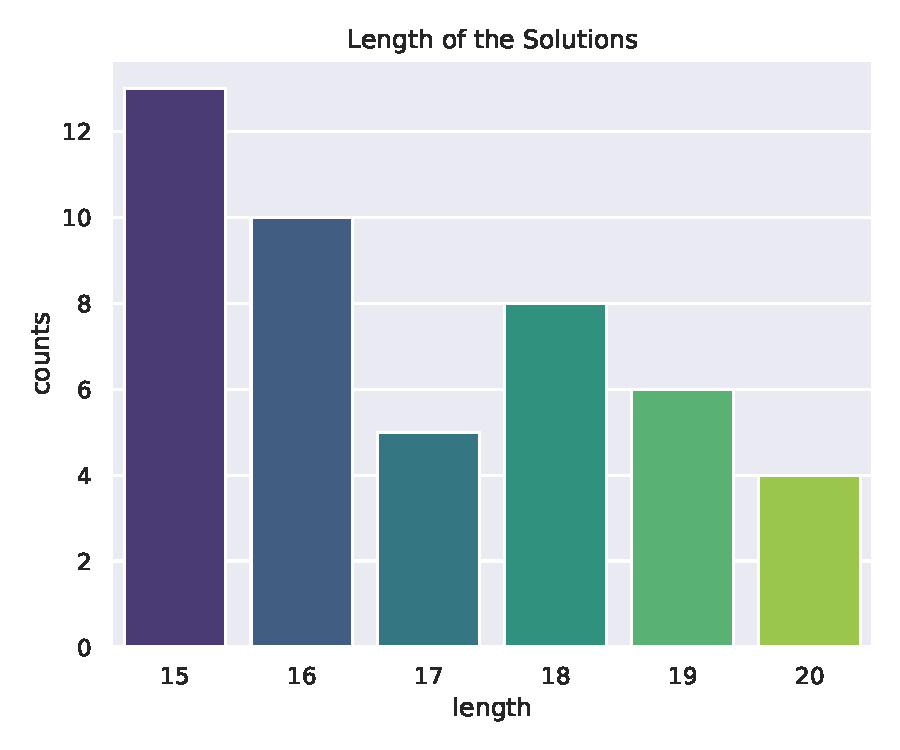
\includegraphics[width=0.4\textwidth]{img/length-solutions}
  \caption{Length of the solutions in the untidied dataset.}
  \label{fig:prelim:length}
\end{figure}
Every observable is characterised by its conformal weight (the \texttt{weight}
column in the dataset), its kind of ``oscillations'' (\texttt{type} variable,
categorical and ordered), its initialisation point (\texttt{init}) and the
truncation levels (from level 2 to level 18).
The objective of the analysis is the prediction of the extrapolation for the
level-$\infty$ truncation hosted in the \texttt{exp} variable of the dataset and which take 3 possible integer values in the range $[-1, 1]$.

\subsection{Input Preparation}\label{sec:prel:prep}

For the analysis we extract each entry of the lists and put it in separate
entry of the dataset: we first artificially insert a new variable labelling the
solution with a number from 0 to 45 and then flatten the dataset over the rows.
This way all columns hold only numerical variables which can be used for
different steps of the analysis.
The tidy dataset is composed of 778 samples over 22 columns (including the
newly created \texttt{solutions} variable).

We then look for duplicates inside the tidy dataset: rows which present exactly
the entries over all the columns, and exclude them from the analysis (we keep
only the first occurrence).
The final version of the dataset holds 732 samples and can be used for the
exploratory data analysis (EDA).


\section{Lumps Solutions}
\subsection{Description}

The dataset is composed of 46 different solutions at different radii.
Each of them is then composed of lists of several observables of different lengths (varying from 15 to 20 entries each, as shown in \Cref{fig:lumps:length}).

\begin{figure}[htbp]
  \centering
  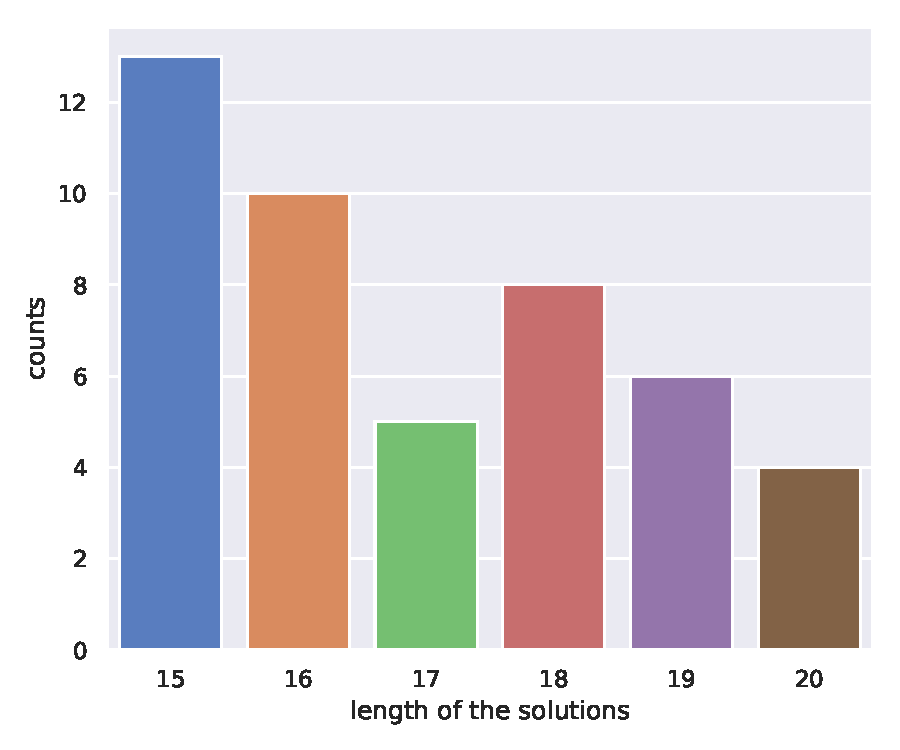
\includegraphics[width=0.6\textwidth]{img/sol_length}
  \caption{Length of the vector-like solutions in the untidied dataset.}
  \label{fig:lumps:length}
\end{figure}

Every observable is characterised by its conformal weight (the \texttt{weight} column in the dataset), its kind of ``oscillations'' (\texttt{type} variable, categorical and ordered), its initialisation point (\texttt{init}) and the truncation levels (from level 2 to level 18).
The \texttt{exp} column contains the label to be predicted from the other variables at finite mass level truncation.
It represents the extrapolation at $\infty$ mass level truncation and takes integer values in the range $[-1, 1]$


\subsection{Preparation}

The entries of the dataset are vector-like objects which need to be tidied before using them for the analysis.
We first artificially insert a new variable (called \texttt{solutions}) to label the 46 different rows of the dataset.
We then flatten the entire dataset over the values in its rows and create a new table containing only numeric entries: the newly formed dataset has 778 rows and 22 columns.

Before proceeding to the analysis we take into account the possibility of relations between the entries and remove the duplicates from the dataset.
In total we remove 46 duplicates corresponding to \SI{6}{\percent} circa of the total dataset.
After this operation the dataset contains 732 rows and it is ready for the \eda.


\subsection{Exploratory Data Analysis}

In the \eda section we study the properties of the tidy dataset.
We focus on outlier detection and correlations between the variables.
We also anticipate that in general we will not use the variables \texttt{init} and \texttt{solutions} since results should not depend on the particular solution or initial value.


\subsubsection{Outliers Detection}

The dataset presents several variables having a very large range of variability and may thus contain a large number of outliers.
As a first step we therefore define the \emph{interquartile} range for each variable and compute the fraction of outlying samples.\footnotemark{}
In general the truncation levels show a high number of outliers (the last truncation level presents \SI{27}{\percent} of outlying values, while others have \SI{20}{\percent} of outliers in average).
\footnotetext{%
  To compute the interquartile range we first compute the 25th and 75th percentiles (i.e.\ the first and third quartiles) of the distribution of each variable.
  The range is then defined as \num{1.5} times the distance between the two quartiles computed from the lower and the upper bounds of the distribution of the values.
}

\begin{figure}[htbp]
  \centering
  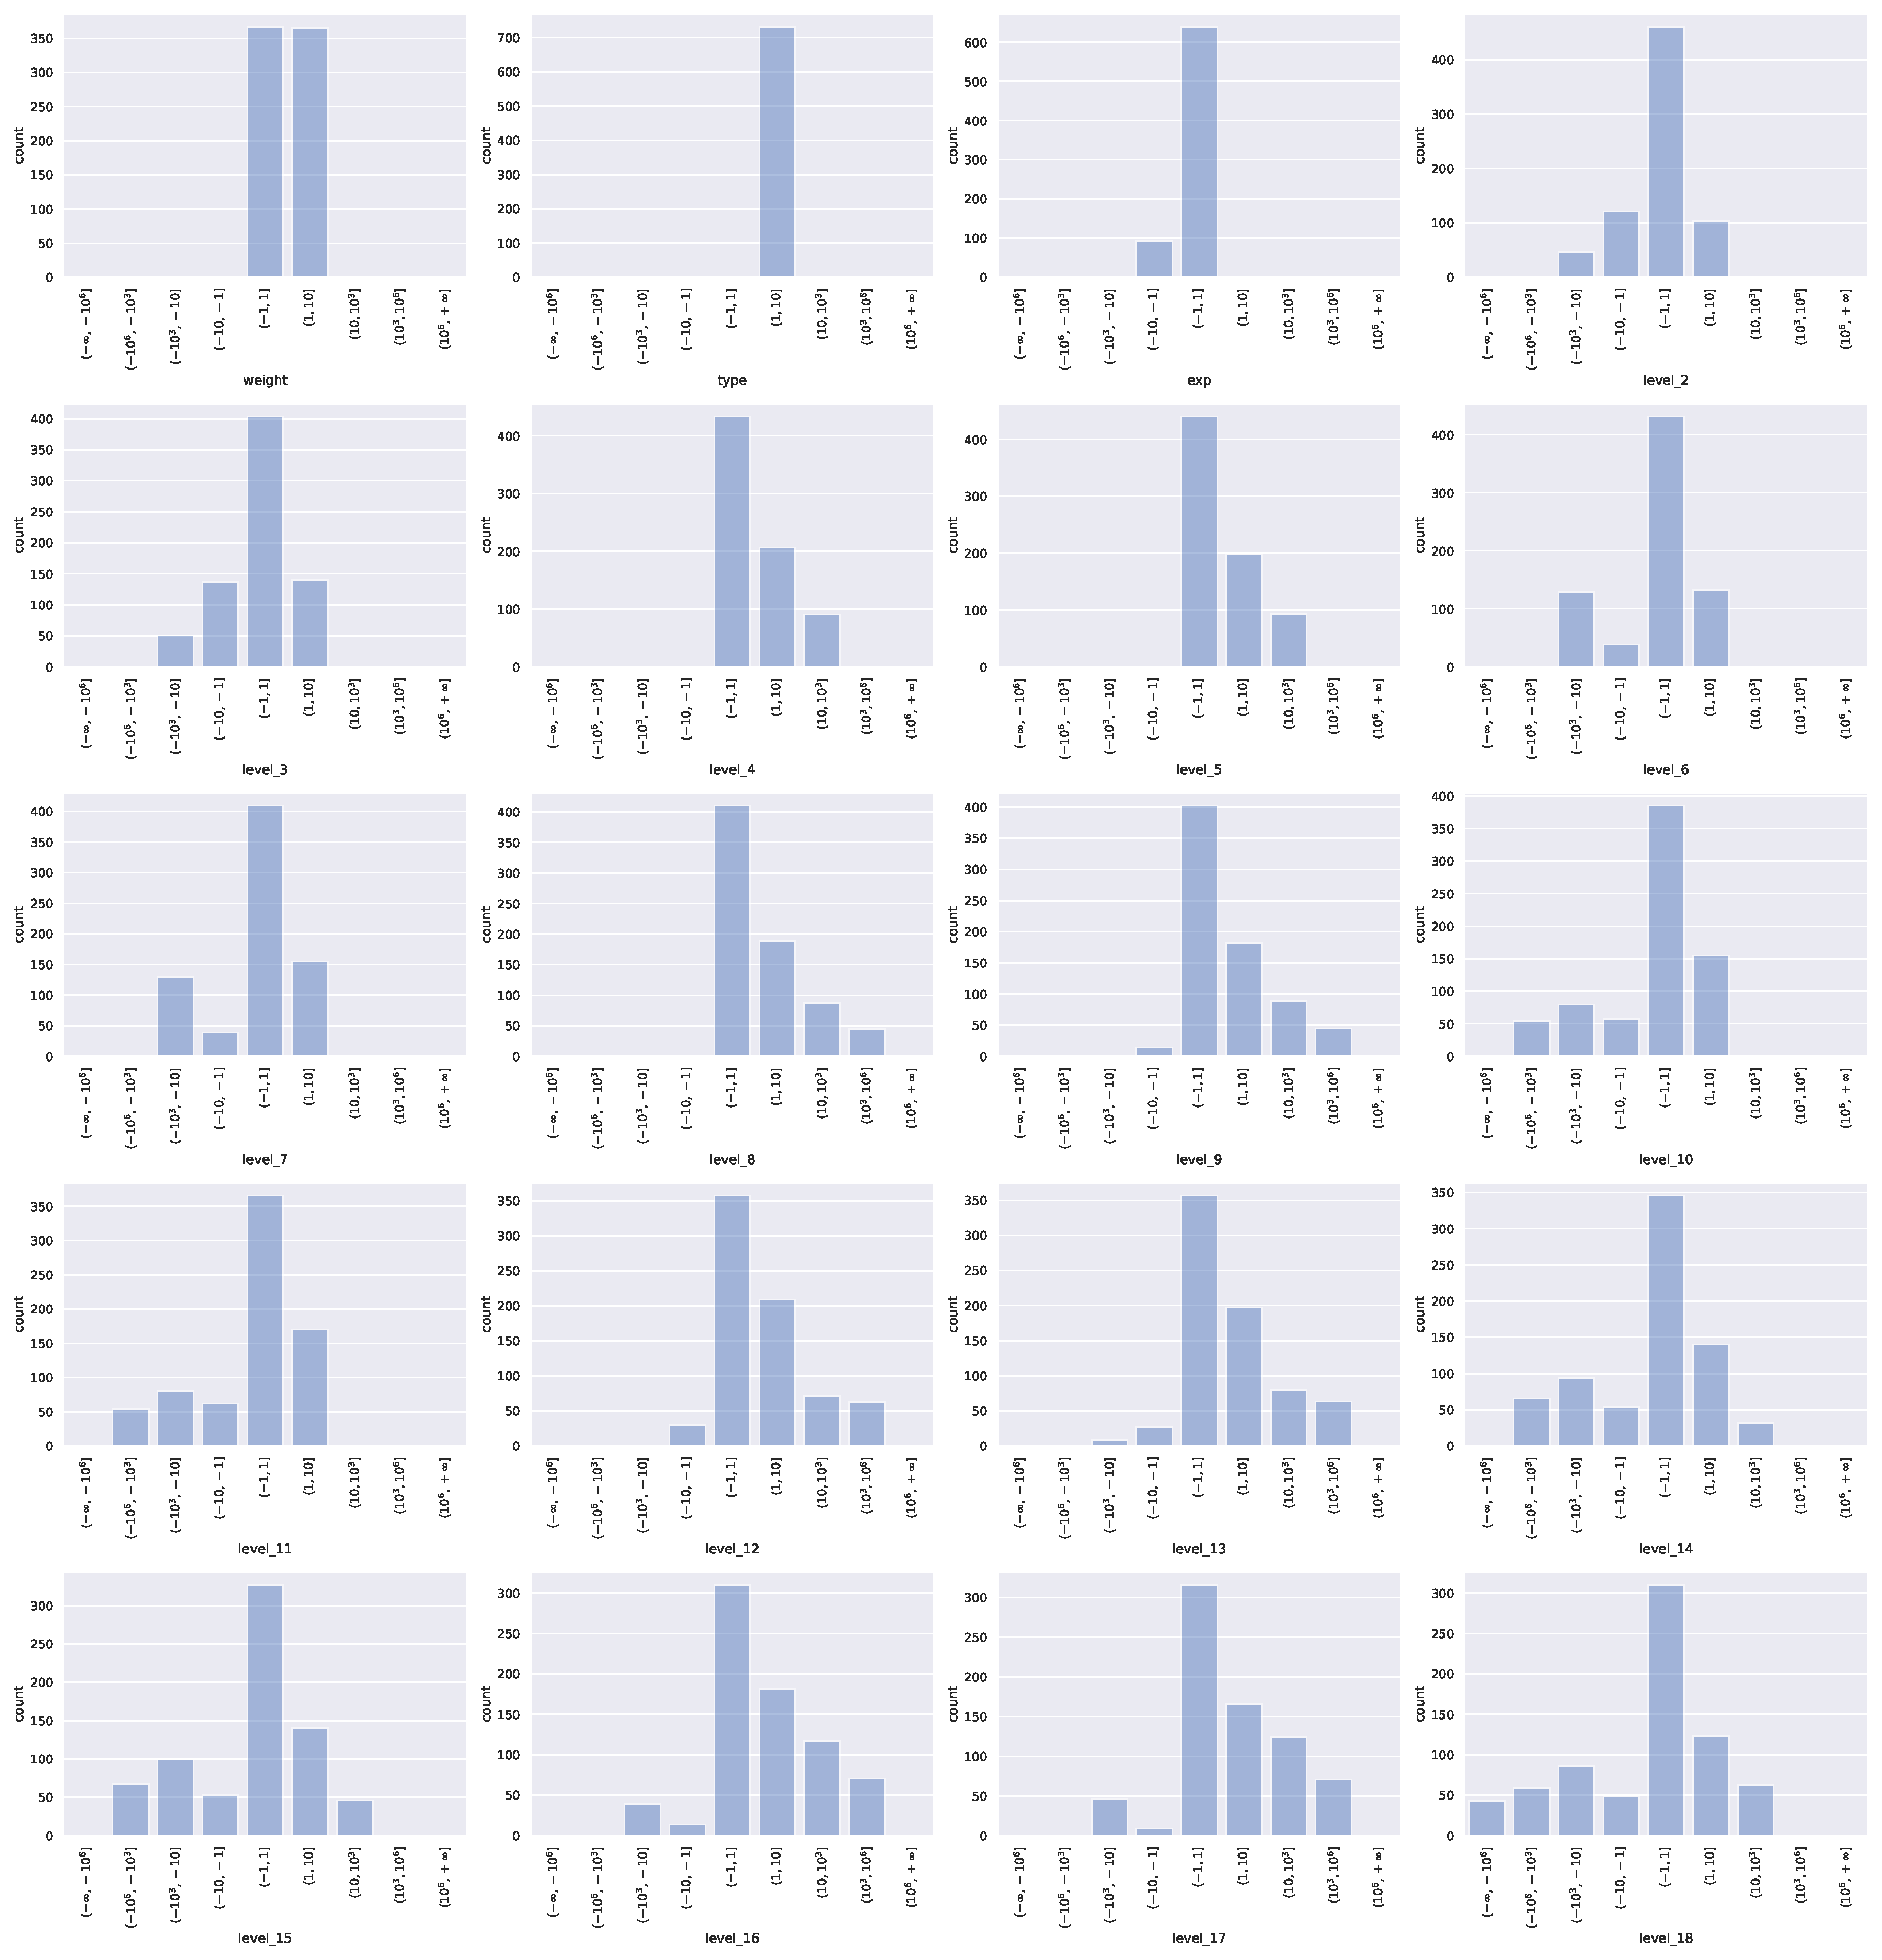
\includegraphics[width=0.6\textwidth]{img/counts_full}
  \caption{Distribution of the values of each variable categorised by order of magnitude.}
  \label{fig:lumps:counts}
\end{figure}

In \Cref{fig:lumps:counts} we show the distribution of the values: in general they are spread across different orders of magnitude and show a tendency to alternate between positive and negative values.
This in turn may cause issues when training \ml algorithms since the very large variance may result in the ``too precise'' determination of the coefficients, ultimately leading to a poor generalisation ability.

However the large number of outliers is mainly due to data corresponding to higher values of \texttt{weight}.
In fact we can separately analyse the dataset for \texttt{weight} $< 1.5$ and \texttt{weight} $\ge 1.5$.
In the first case the values of the variables are in general contained in smaller intervals and present a smaller value of the variance as pictorially shown in \Cref{fig:lumps:box}, where we can see that the variables are in general $\order{1}$ in values.
In the latter the distribution is less uniform and encompasses multiple orders of magnitude (differently from the \texttt{weight} $< 1.5$ case showing a box plot similar to \Cref{fig:lumps:box} does not help in visualising better the situation).

\begin{figure}[htbp]
  \centering
  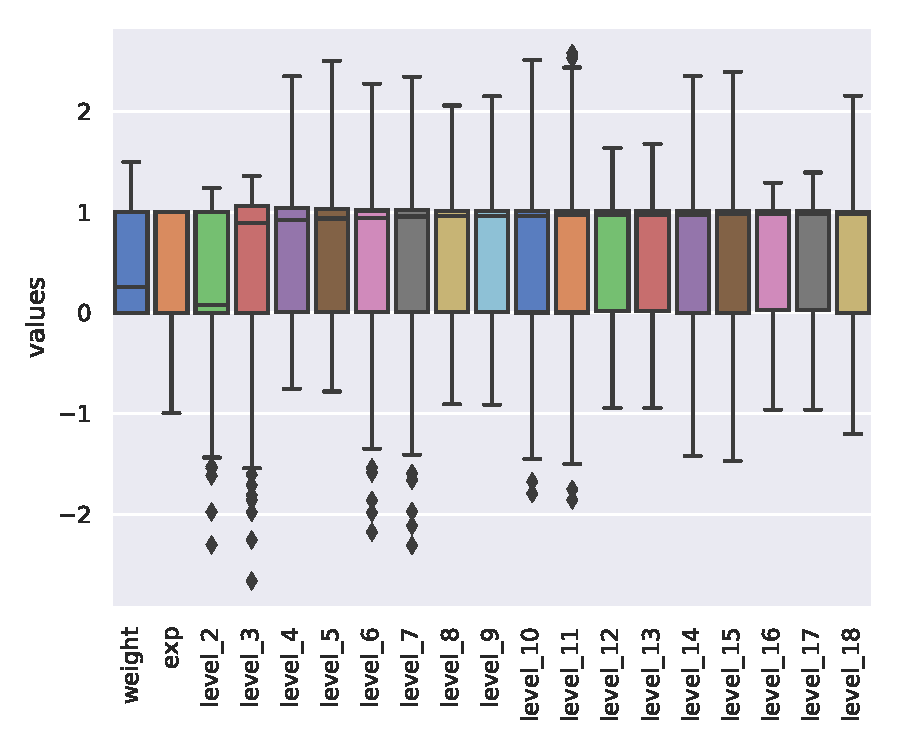
\includegraphics[width=0.6\textwidth]{img/boxplot_low}
  \caption{%
    Boxplot of the values for \texttt{weight} $< 1.5$.
    The coloured boxes represent data between the first and third quartiles (the horizontal line is the median), while the ``whiskers'' show the interquartile range.
    Isolated points are the outliers.
  }
  \label{fig:lumps:box}
\end{figure}

This might be connected to particular relations between the observables. The \eda highlighted some of them (see \Cref{tab:lumps:rel}).
In fact higher weights present only a specific type of oscillation (\texttt{type} is strictly 4), while lower values of \texttt{weight} show that the variables include different kind of oscillations.
However in this case \texttt{type} $= 2$ strictly implies a vanishing weight.

\begin{table}[htbp]
  \centering
  %\resizebox{\textwidth}{!}{%
  \begin{tabular}{@{}cccc@{}}
                     \toprule
                     &               & \multicolumn{2}{c}{\textbf{weight}} \\
  \textbf{weight}    & \textbf{type} & $\mu$             & $\sigma$        \\ \midrule
  \multirow{2}{*}
  {\textgreater 1.5} & 2             & ---               & ---             \\
                     & 4             & 4                 & 2               \\
  \multirow{2}{*}
  {\textless 1.5}    & 2             & 0                 & 0               \\
                     & 4             & 0.6               & 0.5             \\ \bottomrule
  \end{tabular}%
  %}
  \caption{%
    Relations between the \texttt{type} and \texttt{weight} variables.
    In this case $\mu$ is the average value of the \texttt{weight} and $\sigma$ its standard deviation.
  }
  \label{tab:lumps:rel}
\end{table}

Finally in \Cref{fig:lumps:corr} we show the correlation matrices of the variables.
As expected, the truncation levels are strongly correlated among themselves and with the \texttt{weight} variable.
Though milder, there is also a good correlation of the variables with the labels we intend to predict (\texttt{exp}), while the \texttt{type} variable seems to be completely uncorrelated (this may however be due to the fact of being categorical: a linear regression might be more suitable to do statistical inference on it).
Another notable remark is the different behaviour of the correlations between consecutive layers: the large anti-correlations seem to be entirely due to the higher weights, while \texttt{weight} $< 1.5$ seems to imply a correlation only between adjacent couples of levels (e.g.\ 2-3, 4-5, 6-7, etc.) and their replicas at distance 3 (e.g.\ 4-5 with 8-9, 12-13 and 16-17, 6-7 with 10-11, 14-15 and 18, etc.).
This behaviour may point to several possible interpretations.
In particular we see that data is oscillating: going towards larger truncation levels data seem to alternate a behaviour similar to a periodic function (sine or cosine in the particular case) with maxima and minima alternating at constant intervals.
This may become clear when considering the definition of the correlation factor of two variables $X_1$ and $X_2$ given as the ratio between the covariance $\sigma(X_1,X_2) = (X_1 - \bar{X}_1) \cdot (X_2 - \bar{X}_2)$, where $\bar{X}_1$ and $\bar{X}_2$ are the mean of the respective variables, and the product of the separate standard deviations $\sigma(X_1) \sigma(X_2)$).
However we also see that this behaviour is particularly present when considering the full dataset (or just \texttt{weight} $\ge 1.5$) while if we introduce a cut at \texttt{weight} $< 1.5$ the correlation is definitely less marked, though present.

\begin{figure}[htbp]
  \centering
  \begin{subfigure}{0.32\textwidth}
    \centering
    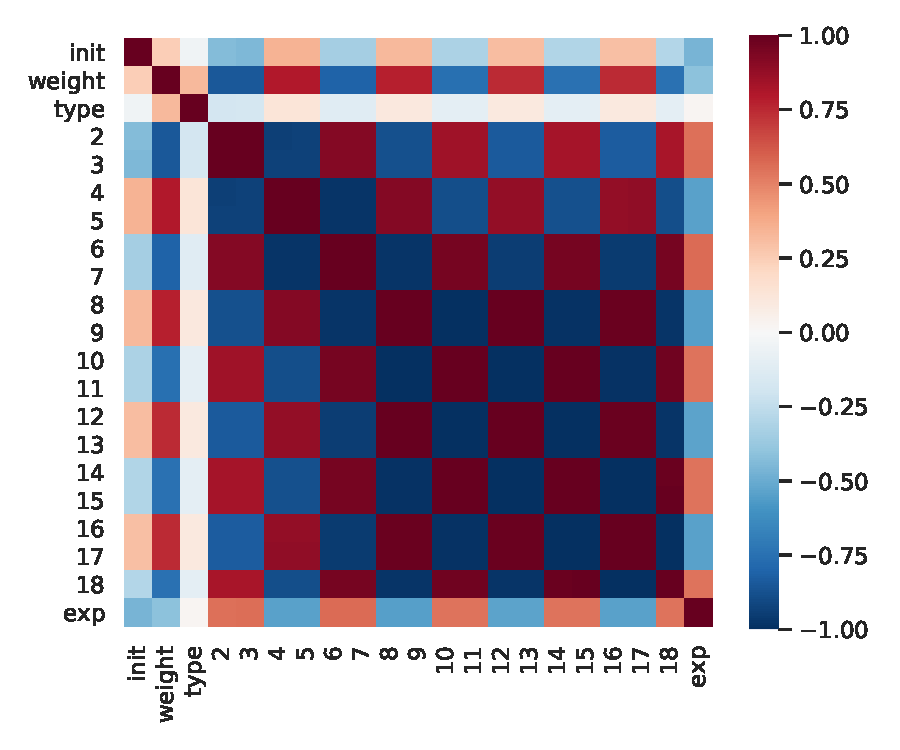
\includegraphics[width=\linewidth]{img/corr_mat_full}
    \caption{Full dataset}
  \end{subfigure}
  \begin{subfigure}{0.32\textwidth}
    \centering
    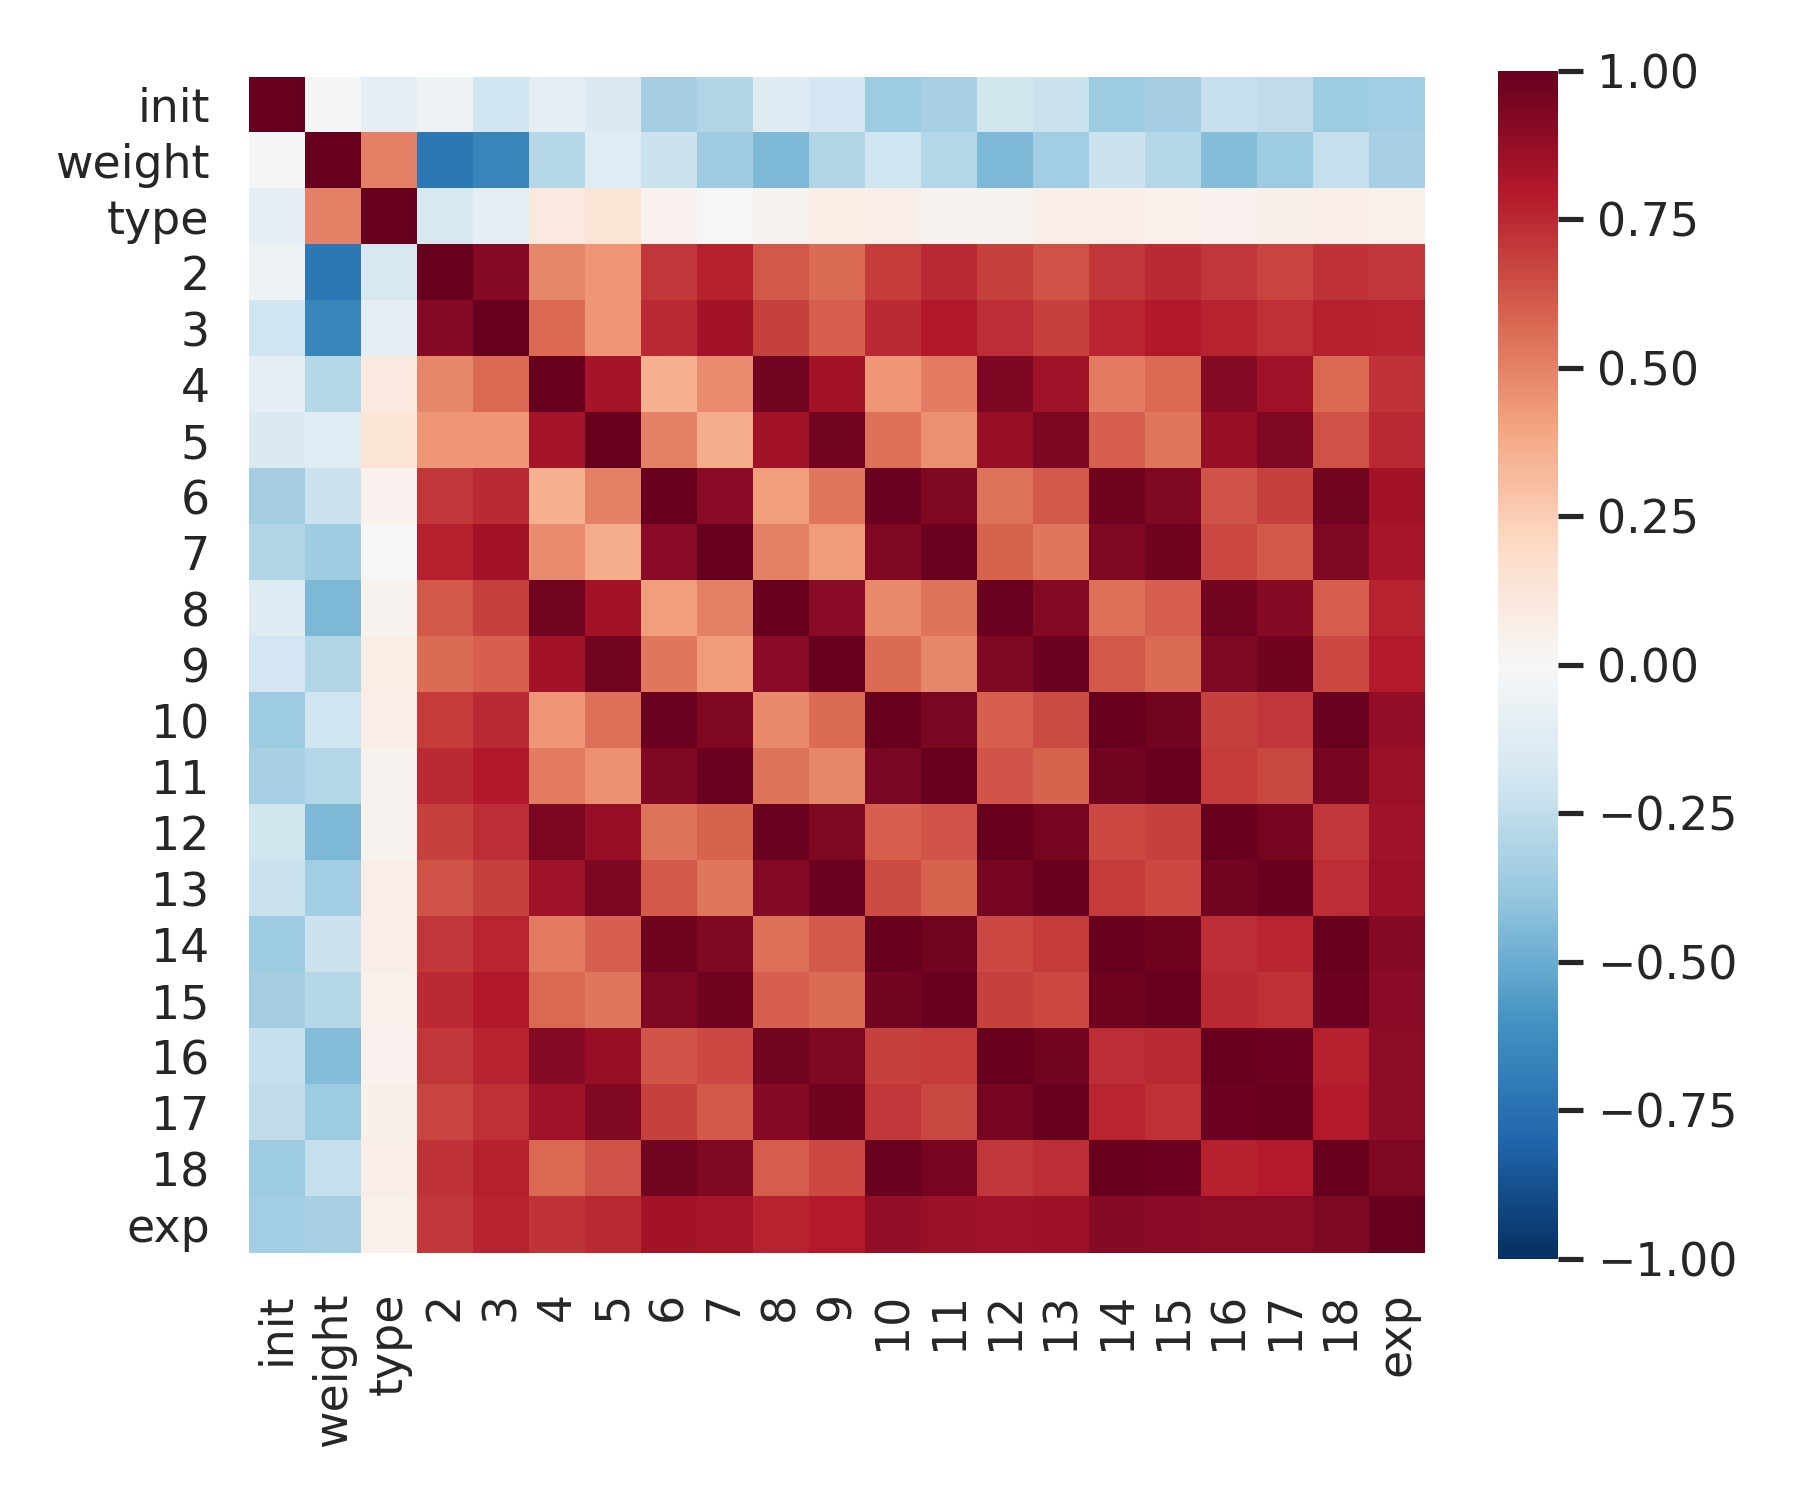
\includegraphics[width=\linewidth]{img/corr_mat_low}
    \caption{\texttt{weight} $< 1.5$.}
  \end{subfigure}
  \begin{subfigure}{0.32\textwidth}
    \centering
    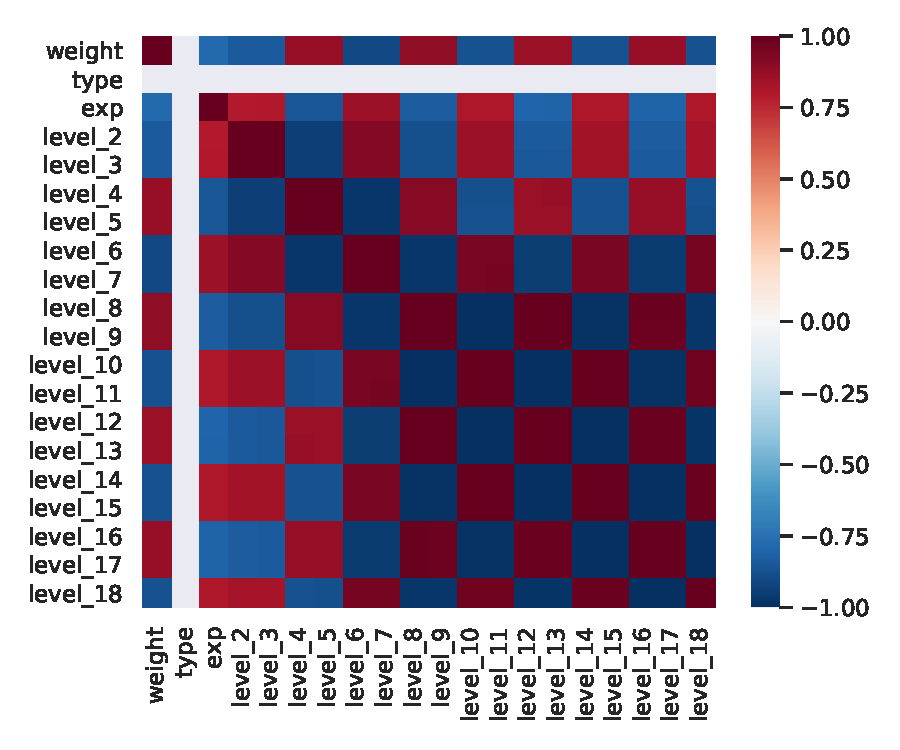
\includegraphics[width=\linewidth]{img/corr_mat_high}
    \caption{\texttt{weight} $\ge 1.5$.}
  \end{subfigure}
  \caption{Correlation matrices of the variables.}
  \label{fig:lumps:corr}
\end{figure}


\subsubsection{Principal Components Analysis}

We perform the Principal Components Analysis (PCA) of the truncation levels to study their properties and their distribution: it encodes the linear variance of the samples by projecting the distribution onto a new system of coordinates trying to maximise such variance in each new axis.
This approach may be interesting both as exploratory analysis and for further directions: we may want to generalise the algorithm to an arbitrary number of truncation levels (and we may want to skip some values).
PCA would then give a solution to always have input of the same size while keeping as much information as possible.

We first study all its components using the Singular Value Decomposition (SVD) of the matrix holding samples over the rows and the truncation levels over the columns (it is a rectangular matrix and as such cannot be strictly diagonalised to perform spectral analysis).
In \Cref{fig:lumps:svd} we show the variance explained by each principal component of the matrix (i.e.\ the fraction of variance of the total set retained by considering only the selected component).

\begin{figure}[htbp]
  \centering
  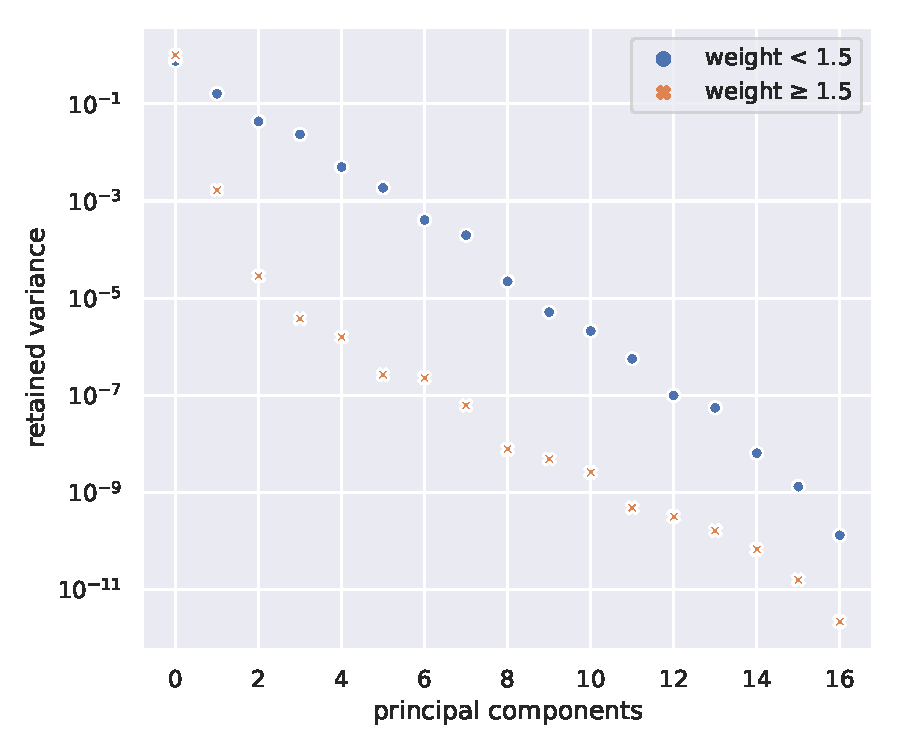
\includegraphics[width=0.6\textwidth]{img/svd}
  \caption{Variance explained by the principal components of the truncation levels (log scale).}
  \label{fig:lumps:svd}
\end{figure}

The analysis was performed splitting the values of the truncation levels over ranges of the \texttt{weight} variable.
The two folds have then been separately scaled: values of \texttt{weight} $< 1.5$ have been standardised (i.e.\ centered and scaled by their standard deviation), while the remaining values have been robustly scaled (i.e.\ centered and scaled by their interquartile) against the outliers present.
The result shows that for lower weights the first two principal components account for more than 90\% of the total variance of the values, while for larger weights almost 100\% of the variance is explained by the first component (in fact the \SI{99}{\percent} of the variance can be reached using 4 components for \texttt{weight} $< 1.5$, while the first component for \texttt{weight} $\ge 1.5$ already contains \SI{99.8}{\percent} of the total variance).
This is a reflection the distribution of the variables in the dataset: larger weights contain a very large amount of outliers and have larger variance with respect to lower weights, thus it might be enough to project the values of the truncation levels over the line which contains most of the deviation to reproduce a meaningful distribution.


\subsubsection{K-Means Clustering}

Finally we perform an unsupervised clustering analysis of the truncation levels.
The main idea is to infer a structure in the data which may be able to ``automatically'' reproduce the labels (i.e.\ the \texttt{exp} column) without regression.
In other words we study the distribution of the truncation levels and fit it in 3 clusters representing the 3 integer values of the labels.\footnotemark{}
\footnotetext{%
  This analysis is strongly related to the finite number of unique values of the label in the dataset.
  It might not be possible to repeat or generalise this procedure to other datasets.
}
In the ideal scenario there should be a 1:1 relation between the labels of the cluster centroids and the labels in the \texttt{exp} variable.
Unfortunately the cluster analysis of the truncation levels over the entire dataset highlighted no particular structure in the data and turned out inconclusive.

We then performed the same analysis splitting the dataset in different ranges of the \texttt{weight} variable, standardising the data for \texttt{weight} $< 1.5$ and robustly scaling (i.e.\ scaling according the interquartile range) samples for which \texttt{weight} $\ge 1.5$.
In \Cref{fig:lumps:kmeans} we used the principal components of the truncation levels to plot the distribution of the clusters and the \texttt{exp} labels.

\begin{figure}[htbp]
  \centering
  \begin{subfigure}{0.45\textwidth}
    \centering
    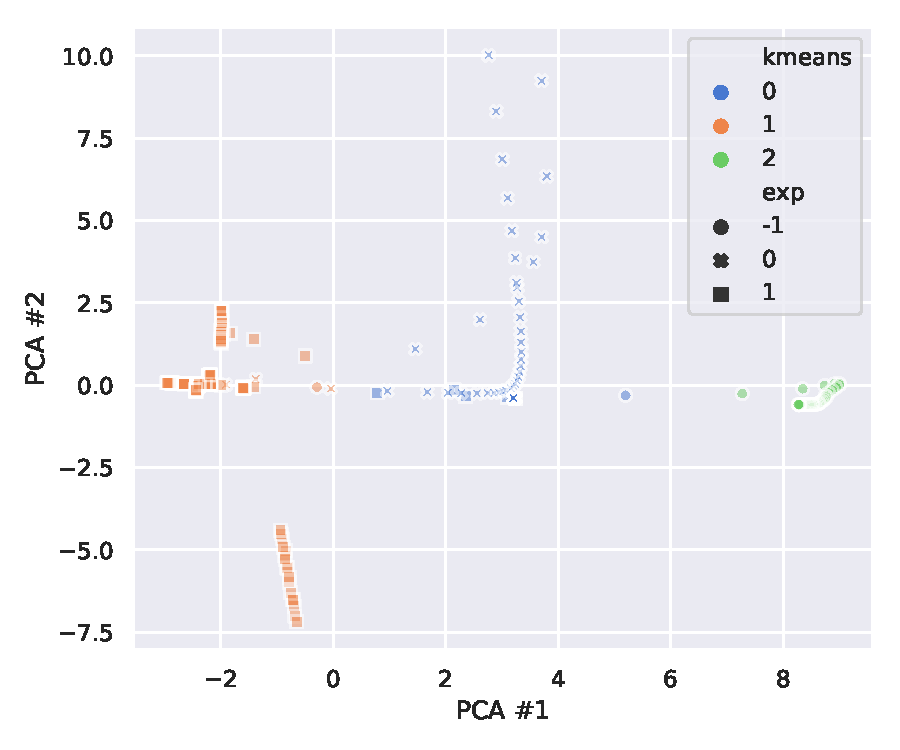
\includegraphics[width=\linewidth]{img/kmeans_low}
    \caption{\texttt{weight} $< 1.5$.}
  \end{subfigure}
  \begin{subfigure}{0.45\textwidth}
    \centering
    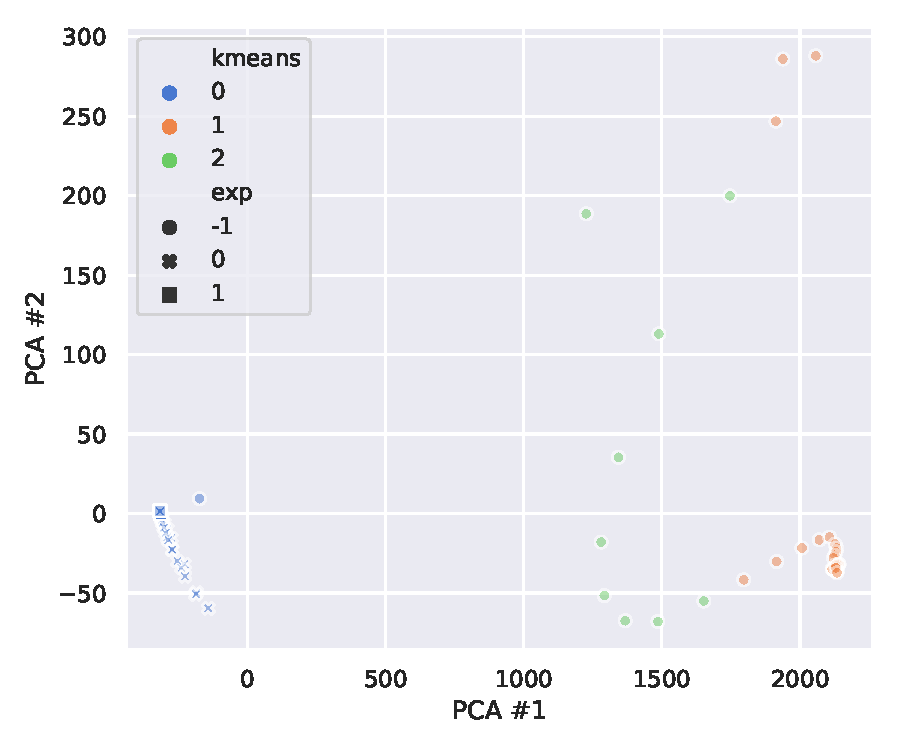
\includegraphics[width=\linewidth]{img/kmeans_high}
    \caption{\texttt{weight} $\ge 1.5$.}
  \end{subfigure}
  \caption{K-Means clusters and \texttt{exp} labels plotted using the principal
  components for visualisation purposes.}
  \label{fig:lumps:kmeans}
\end{figure}

\begin{table}[htbp]
  \centering
  %\resizebox{\textwidth}{!}{%
  \begin{tabular}{@{}ccc@{}}
  \toprule
               & \multicolumn{2}{c}{\textbf{kmeans}} \\
  \texttt{exp} & $\mu$             & $\sigma$        \\ \midrule
  -1           & 1.9               & 0.4             \\
  0            & 0.1               & 0.3             \\
  1            & 0.98              & 0.14            \\ \bottomrule
  \end{tabular}%
  %}
  \caption{Average cluster label for \texttt{weight} $< 1.5$ ($\mu$ is the average value and $\sigma$ its standard deviation).}
  \label{tab:lumps:kmeans}
\end{table}

As we can see, recognising a structure is challenging when \texttt{weight} $\ge 1.5$ and in fact different \texttt{exp} (or ``extrapolation'') labels generally belong to different clusters.
However the case \texttt{weight} $< 1.5$ seems to be more accurate and shows that in general we can recognise a structure in the data.
This is summarised in \Cref{tab:lumps:kmeans} where we show that there is a distinguishable relation between the extrapolation column and the average cluster label in the group
when \texttt{weight} $< 1.5$, while in general there is a superposition of
labels when \texttt{weight} $\ge 1.5$.
Specifically it seems that there are only 2 recognisable clusters since both \texttt{exp} $= 0$ and \texttt{exp} $= 1$ share identically the same cluster label ($\mu = 0$ and $\sigma = 0$).


\subsection{Statistical Inference}

After the \eda we proceed with the study of statistical inference using linear models on the data.
The purpose of the analysis is to better understand the contribution of each variable to the predictions and study the relations among different features.
In the following we will be mainly interested in highlighting the properties of the dataset, while we only marginally mention the predictive ability of the linear model.
We use a simple linear regression without regularisation (using the class \texttt{LinearRegression} in \texttt{Scikit-learn}).

In order to avoid biasing the results, we split the dataset into a training set made of \SI{80}{\percent} of the samples and a development set made of the remaining entries.
The division has been made using the unique values of the \texttt{solutions} column: we first select what solutions to insert in the training and development folds and then assign the corresponding samples to the different sets.
This has the results of keeping similar distributions inside the same set and facilitate the training.\footnotemark{}
\footnotetext{%
  This is again deeply connected with the particular dataset we are using: it might not be possible to generalise such procedure, even though in this case it may help improving the results.
}
We also remove the case \texttt{solutions} $= 0$ (i.e.\ the first entry of the original untidied dataset) because its structure might spoil the generalisation properties since its values are too correlated with the output.

After training the linear model on the training fold, we analyse the outcome on the development set.
With 118 degrees of freedom (\dof) we reach a mean squared error (\mse) of \num{0.16} with a \SI{95}{\percent} confidence interval (\ci) $[0.10, 0.23]$ and a \emph{coefficient of determination} \rr of \num{0.68}.
The interesting part of the analysis is however the \emph{ANalysis Of VAriance} (\anova) of the coefficients summarised in \Cref{tab:lumps:anova} (we do not report also the \ci for brevity).
As we can see the large variance associated with the values of each variable led to a very precise determination of the coefficients (as feared, even too precise).
As a consequence the p-value associated to the observation of more extreme values than those computed here is almost vanishing for all coefficients.
The \texttt{type} variable however has a different behaviour: according to its associated p-value we might consider removing it from the input features.
However such feature, even though irrelevant for the fit, plays an important role when distinguishing higher and lower weights.
We will therefore keep it in the input features to help the algorithms in training (especially the decision trees).\footnotemark{}
\footnotetext{%
  We also repeated the same statistical inference removing the \texttt{type} variable and, as expected, the \anova did not show any difference: all p-values are vanishing in any case.
  However the predictions suffered from the missing variable.
}

\begin{table}[htbp]
  \centering
  %\resizebox{\textwidth}{!}{%
  \begin{tabular}{@{}ccccc@{}}
  \toprule
                     & \textbf{coefficients}       & \textbf{standard error} & \textbf{t statistic} & \textbf{p-value} ($t_{obs} \ge \abs{t}$)  \\
  \midrule
  \texttt{weight}    & 0.109                       & 0.015                   & 7                    & 0.0                                       \\
  \texttt{type}      & 0.03                        & 0.05                    & 0.6                  & 0.5                                       \\
  \texttt{level 2}   & -0.067                      & 0.007                   & -9                   & 0.0                                       \\
  \texttt{level 3}   & 0.135                       & 0.007                   & 20                   & 0.0                                       \\
  \texttt{level 4}   & -0.2955                     & 0.0014                  & $-2 \times 10^2$     & 0.0                                       \\
  \texttt{level 5}   & 0.4161                      & 0.0014                  & $3 \times 10^3$      & 0.0                                       \\
  \texttt{level 6}   & $-2904 \times 10^{-4}$      & $3 \times 10^{-4}$      & $-9 \times 10^3$     & 0.0                                       \\
  \texttt{level 7}   & $4527 \times 10^{-4}$       & $3 \times 10^{-4}$      & $1.5 \times 10^3$    & 0.0                                       \\
  \texttt{level 8}   & $-41345 \times 10^{-5}$     & $6 \times 10^{-5}$      & $-7 \times 10^3$     & 0.0                                       \\
  \texttt{level 9}   & $57675 \times 10^{-5}$      & $6 \times 10^{-5}$      & $1.0 \times 10^3$    & 0.0                                       \\
  \texttt{level 10}  & $-31909 \times 10^{-5}$     & $1.3 \times 10^{-5}$    & $-2 \times 10^4$     & 0.0                                       \\
  \texttt{level 11}  & $43550 \times 10^{-5}$      & $1.3 \times 10^{-5}$    & $3 \times 10^4$      & 0.0                                       \\
  \texttt{level 12}  & $-191313 \times 10^{-6}$    & $3 \times 10^{-6}$      & $-5 \times 10^4$     & 0.0                                       \\
  \texttt{level 13}  & $249714 \times 10^{-6}$     & $3 \times 10^{-6}$      & $6 \times 10^4$      & 0.0                                       \\
  \texttt{level 14}  & $-602220 \times 10^{-7}$    & $8 \times 10^{-7}$      & $-3 \times 10^4$     & 0.0                                       \\
  \texttt{level 15}  & $808300 \times 10^{-7}$     & $8 \times 10^{-7}$      & $4 \times 10^4$      & 0.0                                       \\
  \texttt{level 16}  & $59010 \times 10^{-7}$      & $2 \times 10^{-7}$      & $-5 \times 10^3$     & 0.0                                       \\
  \texttt{level 17}  & $103750 \times 10^{-7}$     & $2 \times 10^{-7}$      & $8 \times 10^3$      & 0.0                                       \\
  \texttt{level 18}  & $43700 \times 10^{-8}$      & $7 \times 10^{-8}$      & $4 \times 10^2$      & 0.0                                       \\
  \bottomrule
  \end{tabular}%
  %}
  \caption{Analysis of the coefficients of the linear model.}
  \label{tab:lumps:anova}
\end{table}


\subsection{Model Dependent Machine Learning Analysis}

As for the previous section, in the \ml analysis we use the tidy dataset without the samples corresponding to \texttt{solutions} $= 0$ to try and retain as much generalisation capability as possible.
We also keep samples corresponding to the same values of \texttt{solutions} in the same set to balance the distribution of the samples as before.
Since the number of samples is small, we will use a single validation set to evaluate the algorithms and perform the optimisation of the hyperparameters.
However, before choosing the validation strategy, we first split the dataset in two folds: the first holds \SI{90}{\percent} of the samples and will be used for training and validation, while the remaining \SI{10}{\percent} will be used for testing.

\begin{figure}[htbp]
  \centering
  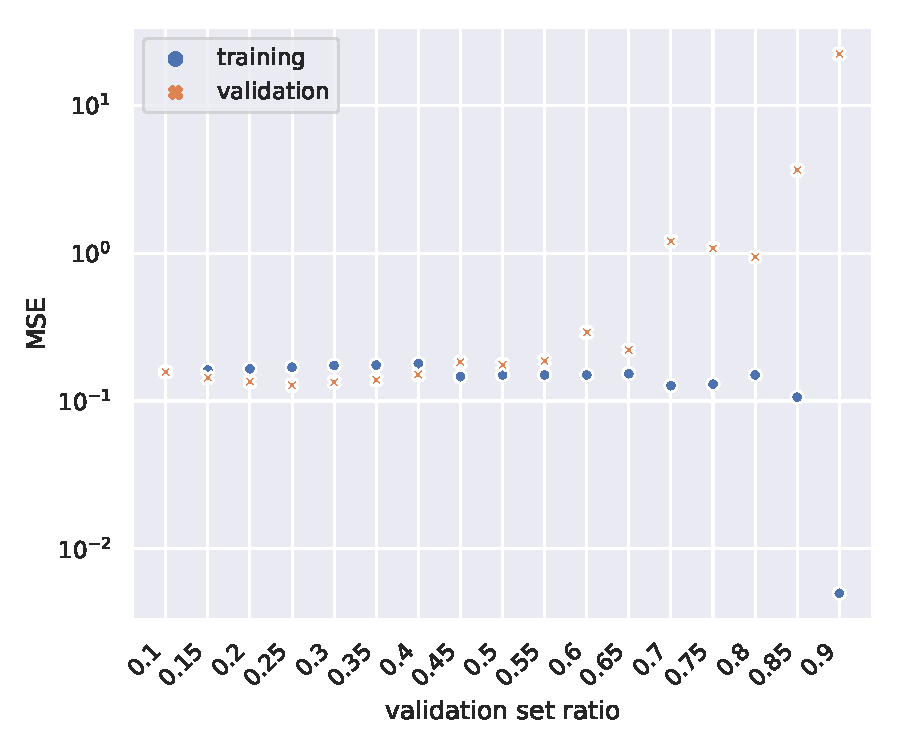
\includegraphics[width=0.6\textwidth]{img/valsize_errors}
  \caption{\mse in training and validation for different validation ratios.}
  \label{fig:lumps:validation_size}
\end{figure}

We then choose the size of the validation set to be around \SI{10}{\percent} of the total training set as it is typical for datasets of this dimension where most of the samples should be assigned to training.

Another motivation for the choice is to try to minimise the error (\mse) made when fitting a linear regression on decreasing size of the set effectively used for training, after removing the validation split: this may clearly not work for anything different from a linear model, but it is however a good starting point.
In \Cref{fig:lumps:validation_size} we show training and validation \mse for different sizes of the validation set (with respect to the total training set).
In order to keep a reasonable amount of samples in the training split and to contain the validation \mse as much as possible, we finally take the already mentioned \SI{10}{\percent} of the unique \texttt{solutions} in the validation set.

\begin{table}[htbp]
\centering
\begin{tabular}{@{}ccc@{}}
\toprule
           & \multicolumn{2}{c}{\textbf{total dataset}} \\
           & \textit{samples}    & \textit{fraction}    \\
\midrule
training   & 584                 & 80\%                 \\
validation & 68                  & 9\%                  \\
test       & 80                  & 11\%                 \\
\bottomrule
\end{tabular}
\caption{Summary of the train/validation/test splits.}
\label{tab:lumps:splits}
\end{table}

In \Cref{tab:lumps:splits} we give a schematic summary of the final choice for training, validation and test sets after assigning the samples corresponding to the chosen \texttt{solutions} in each fold. 

For the \ml analysis we first scale the truncation levels using a robust scaler (such as \texttt{RobustScaler} in \texttt{Scikit-learn}).
We then include also the variables \texttt{weight} and \texttt{type} into the input features.
In \Cref{tab:lumps:preds} we summarise the predictions of different algorithms after optimisation (we use Bayes optimisation techniques to look for the best hyperparameters): \emph{LR} refers to linear regression (with $\ell_2$ regularisation), \emph{l-SVR} is the linear implementation of support vector machines for regression, \emph{r-SVR} uses a \emph{kernel trick} (with a Gaussian function, or \emph{radial} function) for support vectors, \emph{RF} are random forests of decision trees, \emph{GBDT} are gradient boosted decision trees, and finally \emph{ANN} refers to artificial neural networks.\footnotemark{}
\footnotetext{%
  This model is made of 4 hidden layers with \numlist{30;20;20;10} units each and ReLU activation.
  Batch normalisation (with momentum \num{0.99}) follows each layer.
  Dropout layers (with rate \num{0.01}) are used only after the first two layers.
  The output is made of a single unit without activation function.
  We use the \mse as loss function.
  Training is early stopped after 5000 epochs without loss improvement on the validation set and the learning rate (initially set at \num{0.01}) is reduced by a factor \num{0.3} after 2500 epochs without loss improvement.
  While it is in general important to keep track of the models used, the architecture of the aggregate analysis is substantially different, thus making this model not particularly useful.
}

\begin{table}[htbp]
  \centering
  %\resizebox{\textwidth}{!}{%
  \begin{tabular}{@{}ccccc@{}}
  \toprule
                            & \textbf{MSE} & \textbf{95\% C.I.}  & \textbf{MAE} & $r^2$ \\
  \midrule
  \emph{LR ($\ell_2$ reg.)} & 0.16         & (0.07, 0.25)        & 0.3          & 0.68        \\
  \emph{l-SVR}              & 2.4          & (-0.2, 5.1)         & 0.5          & -3.77       \\
  \emph{r-SVR}              & 0.030        & (0.005, 0.046)      & 0.08         & 0.95        \\
  \emph{RF}                 & 0.011        & (-0.003, 0.025)     & 0.04         & 0.98        \\
  \emph{GBDT}               & 0.00085      & (-0.00015, 0.00185) & 0.016        & 1.00        \\
  \emph{ANN}                & 0.00004      & (0.0002, 0.0005)    & 0.005        & 1.00        \\
  \bottomrule
  \end{tabular}%
  %}
  \caption{%
    Summary of the predictions on the test set.
    The number of \dof has been taken to be constant for alla algorithms ($80 - 21 = 59$) as in the linear model for a direct comparison.
  }
  \label{tab:lumps:preds}
\end{table}

As we can see both \emph{GBDT} and \emph{ANN} are able to deliver consistency and precision in the predictions on the test set.
As shown in \Cref{fig:lumps:best} both algorithms perform extremely well on the test set as also the histograms of the residuals in \Cref{fig:lumps:hist}.

\begin{figure}[htbp]
  \centering
  \begin{subfigure}{0.45\textwidth}
    \centering
    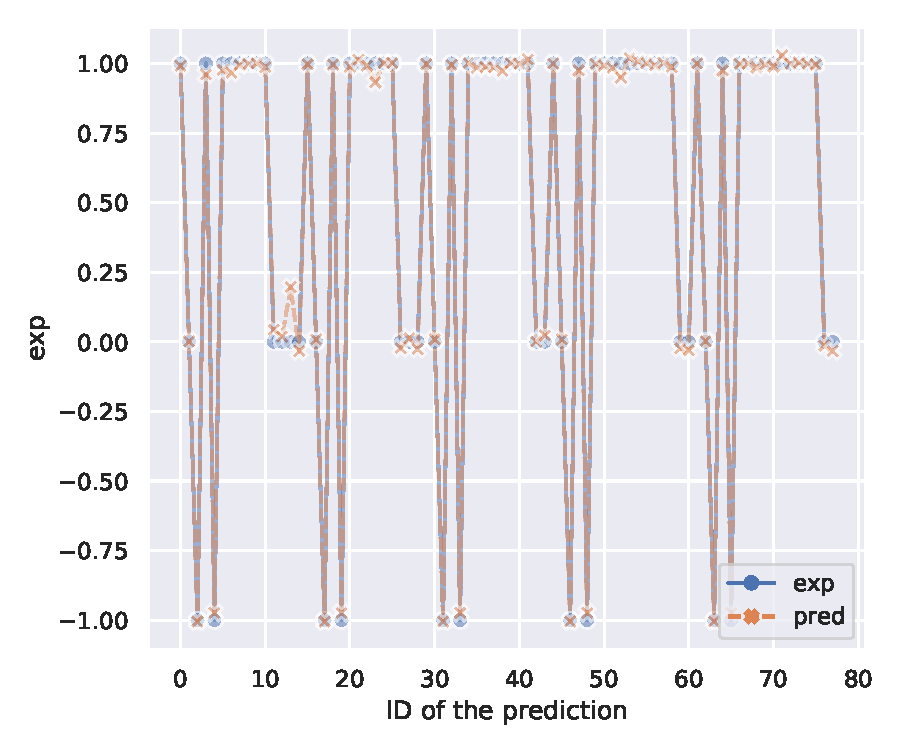
\includegraphics[width=\linewidth]{img/gbdt_lgbmregressor_test_lineplot}
    \caption{\emph{GBDT} predictions and ground truth.}
  \end{subfigure}
  \begin{subfigure}{0.45\textwidth}
    \centering
    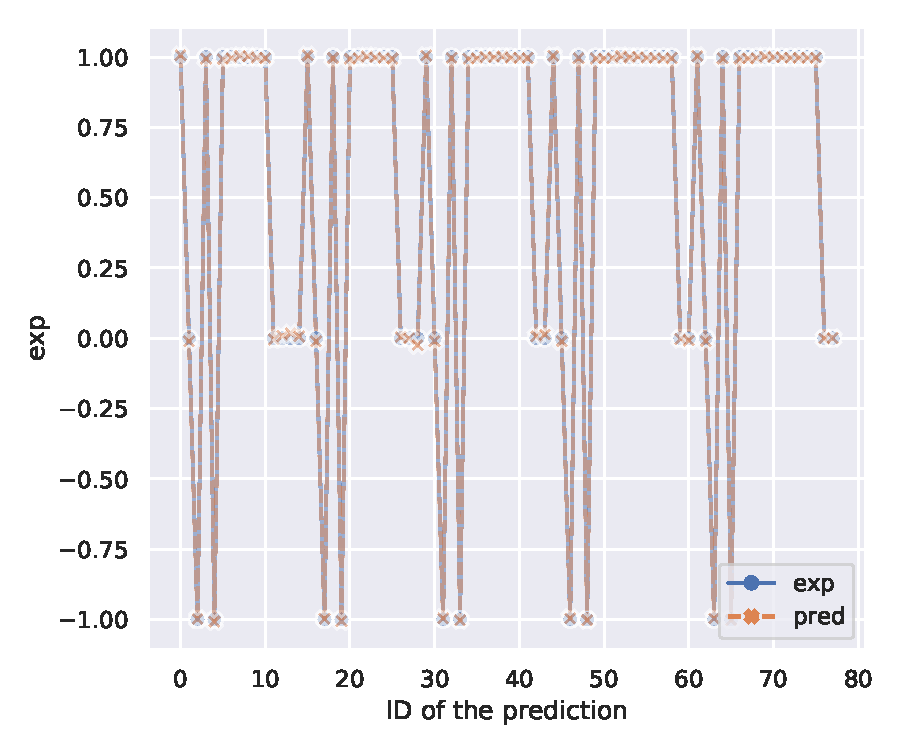
\includegraphics[width=\linewidth]{img/ann_model_test_lineplot}
    \caption{\emph{ANN} predictions and ground truth.}
  \end{subfigure}
  \caption{Predictions and true values for the best algorithms.}
  \label{fig:lumps:best}
\end{figure}

\begin{figure}[htbp]
  \centering
  \begin{subfigure}{0.45\textwidth}
    \centering
    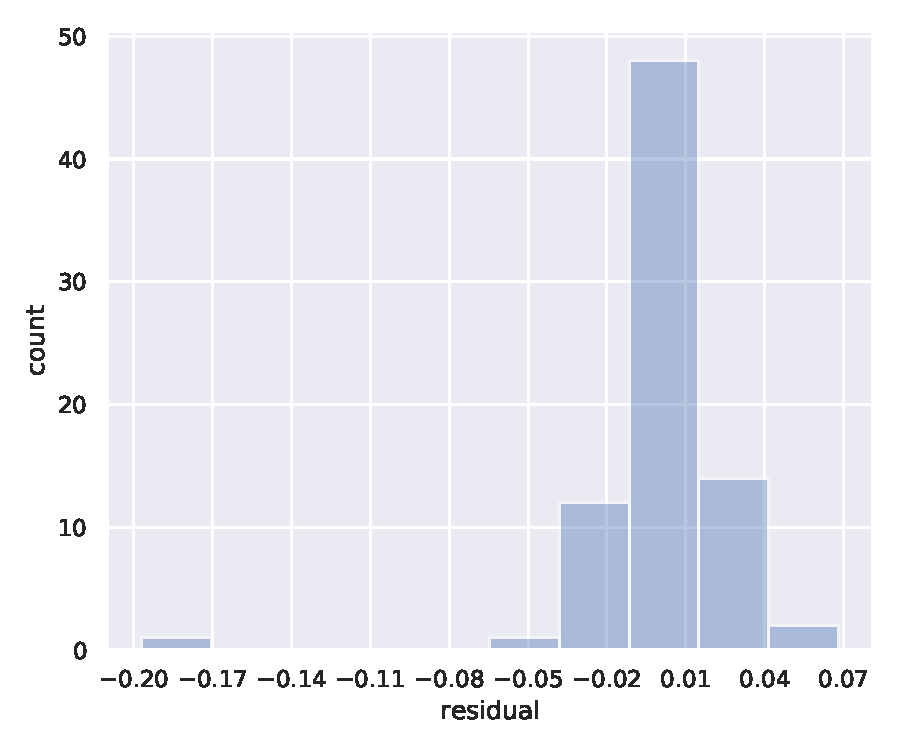
\includegraphics[width=\linewidth]{img/gbdt_lgbmregressor_test_histogram}
    \caption{\emph{GBDT} residuals.}
  \end{subfigure}
  \begin{subfigure}{0.45\textwidth}
    \centering
    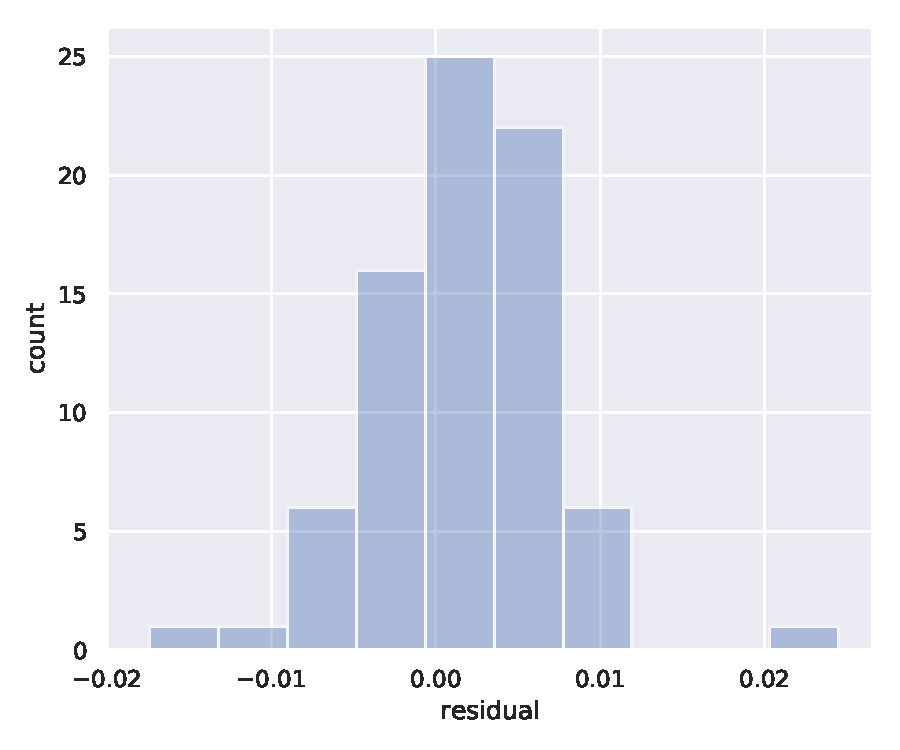
\includegraphics[width=\linewidth]{img/ann_model_test_histogram}
    \caption{\emph{ANN} residual.}
  \end{subfigure}
  \caption{Histogram of the residuals.}
  \label{fig:lumps:hist}
\end{figure}

Given the results of both algorithms we may therefore be interested in seeing the generalisation abilities and the versatility shown by the ANNs on other datasets.
While they both perform well, the ANN might in fact behave better when changing the underlying dataset.
Though extremely good when the training and real world sets have the same distributions, decision trees suffer a lot under small changes in the data: their good performance may therefore be due to the particular range of the label \texttt{exp}.
For generalisation purposes we will therefore focus on the ANN.


\subsubsection{Decision Trees}

After training the algorithms, we now focus on studying the outcome of the decision trees (namely the \emph{RF} and the \emph{GBDT}).
We are interested in better understanding the contributions of each variable to the results through the study of the variable ranking (i.e.\ the feature importances) and the Shapley values.
In \Cref{tab:lumps:hyp} we show the choices of the hyperparameters used for training the decision trees algorithms and which will influence to following analysis.
As we could have imagined, \emph{GBDT}s prefer a larger number of boosting rounds made of small trees, while \emph{RF} prefer a smaller number of fully grown trees.
The relative weight of each sample in the tree changes in both implementations of the decision trees and is definitely more relevant when the trees are smaller (i.e.\ in the \emph{GBDT}).
Both $\ell_1$ (\texttt{reg\_alpha}) and $\ell_2$ (\texttt{reg\_lambda}) regularisation have been used to produce the predictions.

\begin{table}[htbp]
  \centering
  \begin{tabular}{@{}lrr@{}}
      \toprule
      \textbf{hyperparameters}    & \textbf{RF} & \textbf{GBDT} \\
      \midrule
      \texttt{num\_leaves}        & 70          & 10            \\
      \texttt{max\_depth} 	  & 500         & 25            \\
      \texttt{learning\_rate}     & ---         & 0.1           \\
      \texttt{n\_estimators} 	  & 50          & 1590          \\
      \texttt{subsample} 	  & 0.99        & 0.66          \\
      \texttt{colsample\_bytree}  & 1.00        & 1.00          \\ \texttt{min\_child\_weight} & $10^{-6}$   & $10^{-3}$     \\
      \texttt{reg\_alpha} 	  & 0.1         & 1.0           \\
      \texttt{reg\_lambda}        & 0.12        & 1.0           \\
      \bottomrule
  \end{tabular}
  \caption{Hyperparameters used by \emph{RF} and \emph{GBDT}.}
  \label{tab:lumps:hyp}
\end{table}

The importance of the features is a key property of the decision trees and visually summarises the impact that each feature has on the final prediction: variables with higher importance can be found in the first branches of the trees because they are responsible for the main choices of the algorithm, while more negligible features provide the necessary refinement.
The Shapley values are somewhat related and derive from a game theoretic approach to the decision trees: these values encode how a certain feature is influencing the final result, whether by dragging its value with respect to average of the predictions or by pushing it beyond it.
In other words, feature importances show how much (as a percentage of the final prediction) a variable is relevant for the algorithm and the Shapley values show if there are variables which tend to drive the results towards a
particular value (by computing the interaction between Shapley values we can also try to recognise inter-dependencies inside the trees which may be worth analysing further.

\begin{figure}[htbp]
  \centering
  \begin{subfigure}{0.45\textwidth}
    \centering
    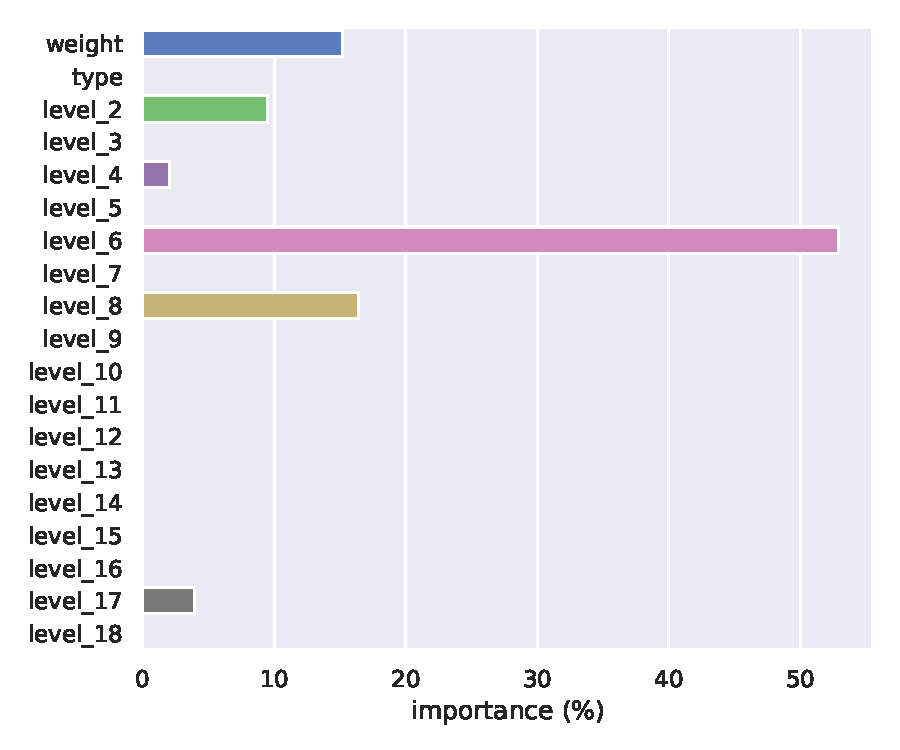
\includegraphics[width=\linewidth]{img/rnd_for_rank}
    \caption{Variable ranking.}
  \end{subfigure}
  \begin{subfigure}{0.45\textwidth}
    \centering
    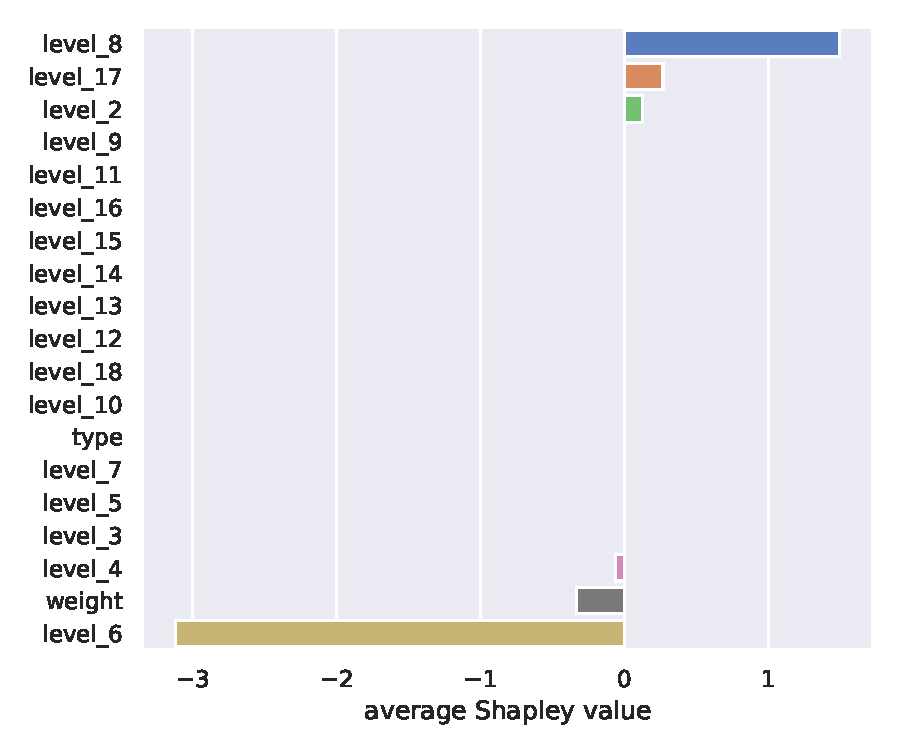
\includegraphics[width=\linewidth]{img/rnd_for_shap}
    \caption{Shapley values.}
  \end{subfigure}
  \caption{Feature importances and Shapley values of the \emph{RF}.}
  \label{fig:lumps:rnd_for}
\end{figure}

In \Cref{fig:lumps:rnd_for} we show the variable ranking and the Shapley values for the \emph{RF} algorithm.
The first plot sow that RF rely on a particular truncation level (level-6 to be specific) to produce the predictions, while other features contribute in a less relevant manner.
The average Shapley values (second plot) show that most features give a comparable contribution to the prediction, exception made for the mass truncation at level-6 and level-7 which seem to drive the final result in a more direct way (according to \Cref{fig:lumps:counts} they are among the highly unbalanced values, which may be a reason of such behaviour).

\begin{figure}[htbp]
  \centering
  \begin{subfigure}{0.45\textwidth}
    \centering
    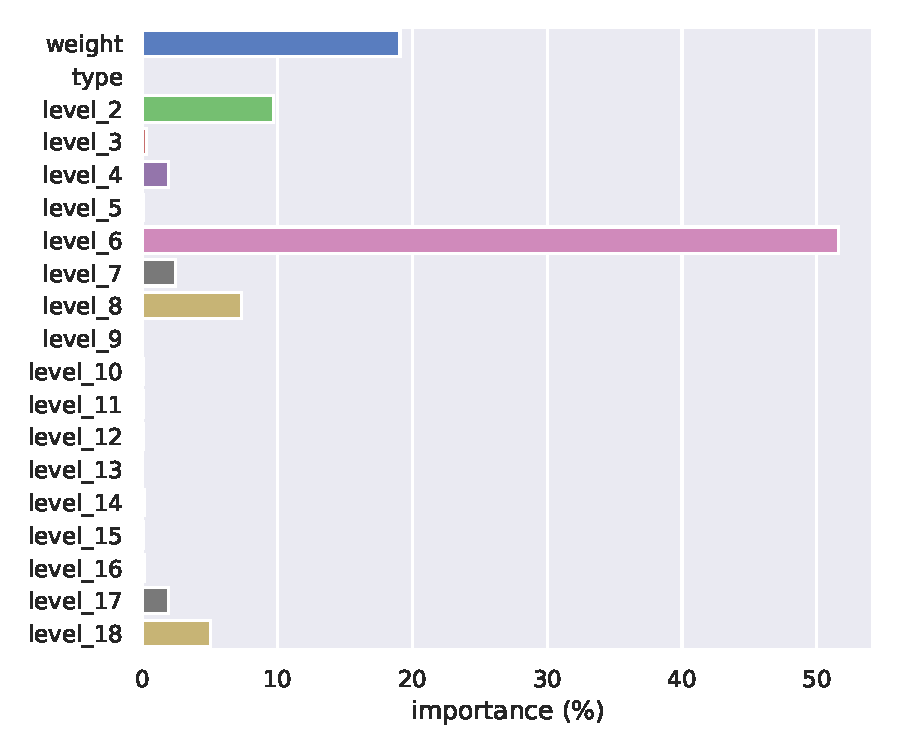
\includegraphics[width=\linewidth]{img/grd_bst_rank}
    \caption{Variable ranking.}
  \end{subfigure}
  \begin{subfigure}{0.45\textwidth}
    \centering
    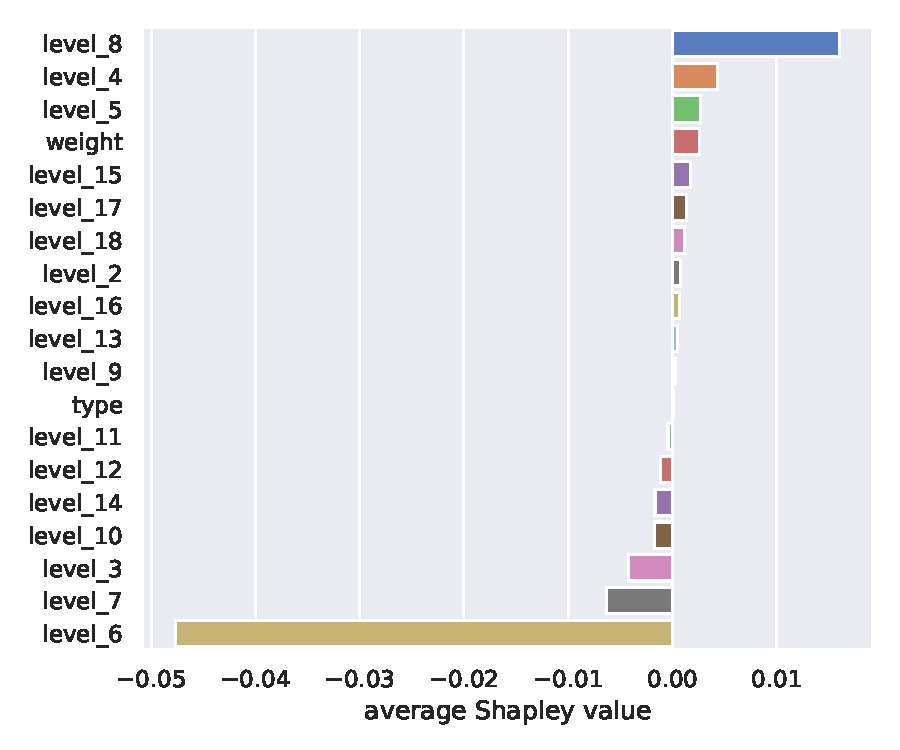
\includegraphics[width=\linewidth]{img/grd_bst_shap}
    \caption{Shapley values.}
  \end{subfigure}
  \caption{Feature importances and Shapley values of the \emph{GBDT}s.}
  \label{fig:lumps:grd_bst}
\end{figure}

In \Cref{fig:lumps:grd_bst} we finally show the same plot for the \emph{GBDT}s.
Differently from the \emph{RF}, \emph{GBDT}s seem to rely almost entirely on the 6th truncation level and \texttt{weight} discrimination of the samples.
In both cases the algorithms seem to ignore almost completely the categorical variable \texttt{type} (possibly it could have been removed but the corresponding Shapley value shows that its relevance is so marginal that the result would not have changed).

We notice that the scale of the Shapley values is very different between \emph{RF} and \emph{GBDT}: this is due to the fact that in this case the boosting procedure may be more robust against the large variability of the dataset, showing that in the \emph{GBDT} case the trees are more balanced.
Ultimately this is also a consequence of the different order of magnitude of the \mse associated to \emph{RF} and \emph{GBDT}, the latter being an entire order of magnitude more precise than the former.

We also performed this type of analysis on \emph{GBDT} successively removing different subsamples of the features in the attempt to better understand the presence of one feature with a very high importance with respect to all others.
Results showed that whatever the subsample of features, the algorithm always chooses the 3rd to 5th level truncation level as most important: after guessing the behaviour based on the first few truncation levels, the algorithm finally predict the label using one particular feature (\texttt{level 6} in the case shown in the figures) and finally refines it using the last truncations levels.


\subsubsection{Double Lumps}

As a test of the generalisation ability of the algorithms, we perform predictions on double lumps solutions using the algorithms trained in the previous section (i.e.\ we do not perform again the optimisation and training procedure).
The dataset used is made of 20 entries with the same columns as the previous solutions.

Before making predictions, we scale the truncation levels using the same robust scaler we used in the previous section.
The predicted labels are then directly comparable with the real values.
In \Cref{tab:lumps:dlumps} we show the complete list of the predictions made on the double lumps.\footnotemark{}
\footnotetext{%
  Since the performance has been in general very poor, we removed the predictions using \emph{l-SVR} as model.
}
We kept \texttt{weight} and \texttt{type} to label each solution (we dropped the truncation levels for brevity).
Finally we pictorially show the predictions in \Cref{fig:lumps:dlump_preds}: as imagined, decision trees kept the prediction interval $[-1, 1]$ as the original dataset on which they were trained, while the ANN have extrapolated more.

\begin{figure}[htbp]
  \centering
  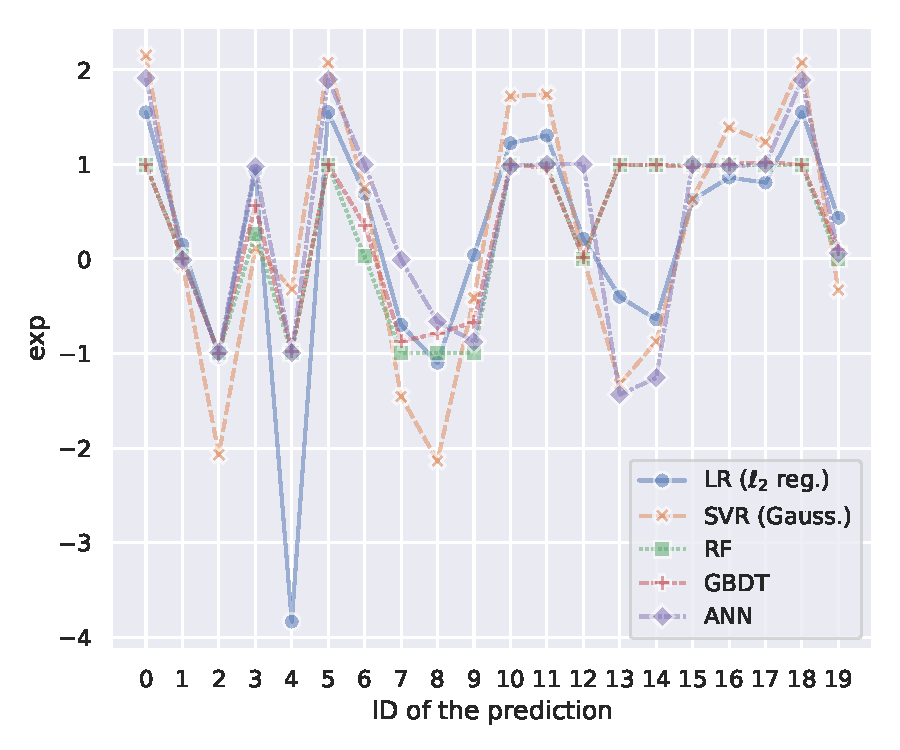
\includegraphics[width=0.6\textwidth]{img/dlumps_pred}
  \caption{Double lumps predictions.}
  \label{fig:lumps:dlump_preds}
\end{figure}

\begin{table}[htbp]
  \centering
  %\resizebox{\textwidth}{!}{%
  \begin{tabular}{@{}ccccccc@{}}
  \toprule
  \textbf{weight} & \textbf{type} & \textbf{exp (LR)} & \textbf{exp (r-SVR)} & \textbf{exp (RF)} & \textbf{exp (GBDT)} & \textbf{exp (ANN)} \\ \midrule
  0.000000        & 2             & 1.551467          & 2.153519             & 0.989096          & 0.994209            & 1.910616           \\
  0.000000        & 2             & 0.148665          & -0.054234            & 0.026711          & 0.008819            & -0.010774          \\
  1.000000        & 4             & -1.036330         & -2.071016            & -0.991434         & -0.998615           & -0.987881          \\
  4.000000        & 4             & 0.930320          & 0.114937             & 0.264700          & 0.563773            & 0.978944           \\
  9.000000        & 4             & -3.834771         & -0.322144            & -0.991861         & -0.974030           & -0.990880          \\
  0.000000        & 4             & 1.552892          & 2.075871             & 0.989096          & 0.995166            & 1.894776           \\
  0.027778        & 4             & 0.690183          & 0.749930             & 0.026711          & 0.358236            & 0.998884           \\
  0.111111        & 4             & -0.696637         & -1.455321            & -0.991434         & -0.869838           & -0.007325          \\
  0.250000        & 4             & -1.099292         & -2.137033            & -0.991434         & -0.787782           & -0.664277          \\
  0.444444        & 4             & 0.040714          & -0.412954            & -0.991434         & -0.667371           & -0.874694          \\
  0.694444        & 4             & 1.223861          & 1.721034             & 0.989096          & 1.000537            & 0.981812           \\
  1.000000        & 4             & 1.305418          & 1.741227             & 0.989096          & 0.962043            & 1.004753           \\
  1.361111        & 4             & 0.213720          & 0.014285             & 0.002803          & 0.019858            & 1.000996           \\
  1.777778        & 4             & -0.400493         & -1.323758            & 0.997782          & 0.996645            & -1.434201          \\
  2.250000        & 4             & -0.639370         & -0.874269            & 0.997782          & 0.995911            & -1.257340          \\
  2.777778        & 4             & 0.625367          & 0.635726             & 0.997782          & 0.971987            & 0.997438           \\
  3.361111        & 4             & 0.860903          & 1.392883             & 0.997782          & 1.002204            & 0.979112           \\
  4.000000        & 4             & 0.807342          & 1.234534             & 0.989096          & 1.023945            & 0.998200           \\
  0.000000        & 4             & 1.552892          & 2.075871             & 0.989096          & 0.995166            & 1.894776           \\
  2.250000        & 4             & 0.434775          & -0.329326            & 0.002803          & 0.101149            & 0.059882           \\ \bottomrule
  \end{tabular}%
  %}
  \caption{Predictions on the double lumps set.}
  \label{tab:lumps:dlumps}
\end{table}

We finally compare the results of the predictions of the double lumps with the extrapolated labels.
In order to keep only the most reliable results, we limit the predictions to \texttt{weight} $< 1.5$.
In \Cref{tab:lumps:double_metrics} we summarise the results which showed a good result for the \emph{r-SVR} algorithm with $\rr = 0.96$.

\begin{table}[htbp]
  \centering
  %\resizebox{\textwidth}{!}{%
  \begin{tabular}{@{}cccc@{}}
  \toprule
               & \mse & \mae & \rr   \\ \midrule
  \emph{LR}    & 0.3  & 0.5  & 0.85 \\
  \emph{r-SVR} & 0.10 & 0.3  & 0.96 \\
  \emph{RF}    & 0.6  & 0.7  & 0.72 \\
  \emph{GBDT}  & 0.6  & 0.7  & 0.72 \\
  \emph{ANN}   & 0.4  & 0.5  & 0.81 \\ \bottomrule
  \end{tabular}%
  %}
  \caption{Metrics computed on the double lumps with \texttt{weight} $< 1.5$.}
  \label{tab:lumps:double_metrics}
\end{table}



\section{WZW Model}
\subsection{Description and Preparation}

The main difference from the previous dataset is represented by the presence of complex ($\C$) values of certain variables.
In particular the truncation levels and the \texttt{exp} label have all complex values.
Moreover there are additional variables which label the solutions such as the level \texttt{k} and the quantum numbers \texttt{j} and \texttt{m} referring to the \SU{2} representation of the solution.

As in the previous case, the dataset is made of 46 vector-like entries which have to be flattened in the tidy version of the dataset.
The length of the solutions is different in each entry and the number of solutions for different sizes is summarised in \Cref{fig:wzw:length}.

\begin{figure}[htbp]
  \centering
  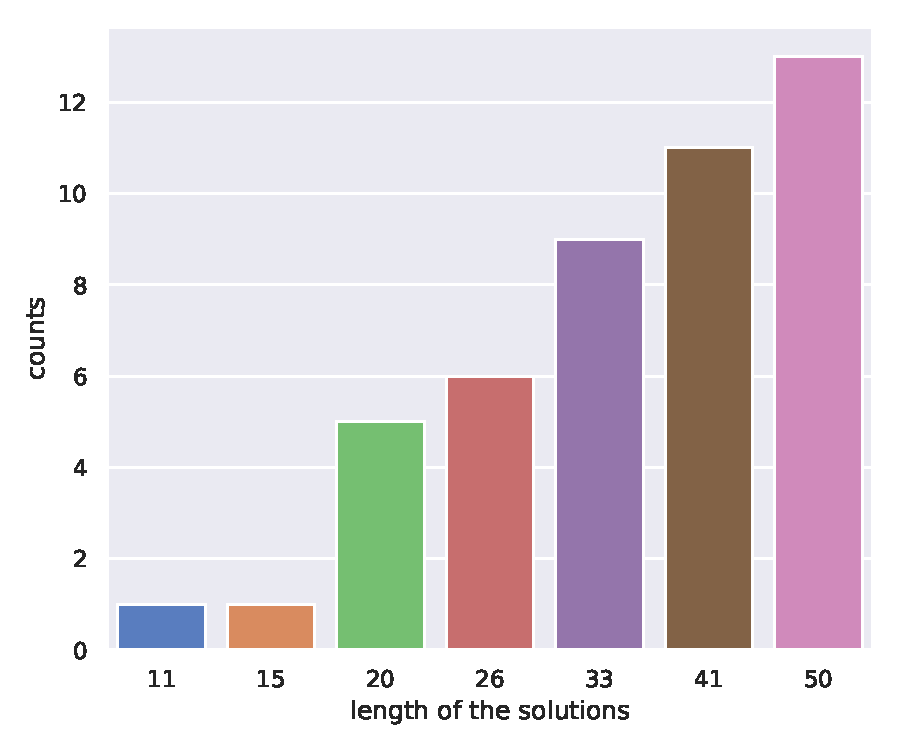
\includegraphics[width=0.6\textwidth]{img/re_sol_length}
  \caption{Length of various solutions.}
  \label{fig:wzw:length}
\end{figure}

In this case the available truncation levels start from the 2nd to the 14th, but since the last 4 levels have mostly empty values we drop them and stop at level 10.

We finally prune the dataset of the duplicates and drop 33 entries (or roughly \SI{2}{\percent} of the total dataset) which are identical over all the variables.

The tidy dataset has therefore 1680 row entries and spans 25 variables including the real and imaginary parts of the label \texttt{exp}, the real and imaginary parts of the truncation levels, \texttt{k}, \texttt{weight}, \texttt{j} and \texttt{m}.


\subsection{Exploratory Data Analysis}

In the exploratory data analysis we mainly focus on the distribution of the values and patterns in the data.


\subsubsection{Distribution of the Data}

Looking at the summary of the data we recognise immediately some properties of the solutions.
In \Cref{fig:wzw:summary} we show a visual summary of the statistics associated with the variables labelling each solutions (without the truncation levels which will be studied later).
For instance we immediately recognise that both sum and average of the quantum number \texttt{m} are vanishing, together with possible correlations between \texttt{k}, \texttt{j} and \texttt{weight}.\footnotemark{}
\footnotetext{%
  In fact \texttt{weight} $= \frac{j(j+1)}{k + 2)}$.
}

\begin{figure}[htbp]
  \centering
  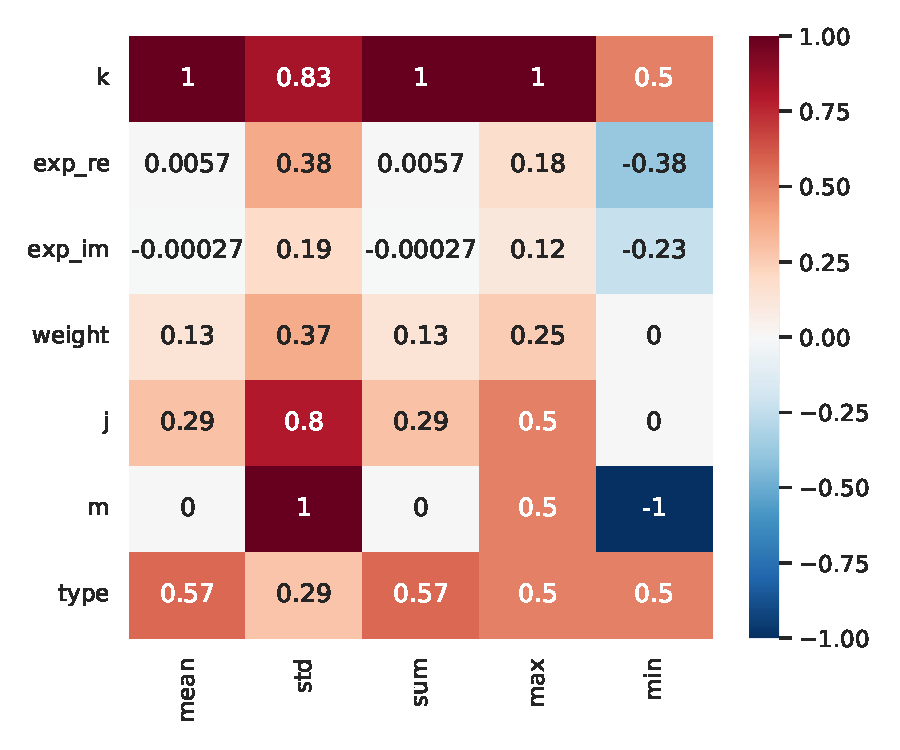
\includegraphics[width=0.6\textwidth]{img/oth_nodup_summary_norm}
  \caption{Visual representation of the summary statistics.}
  \label{fig:wzw:summary}
\end{figure}

\begin{figure}[htbp]
  \centering
  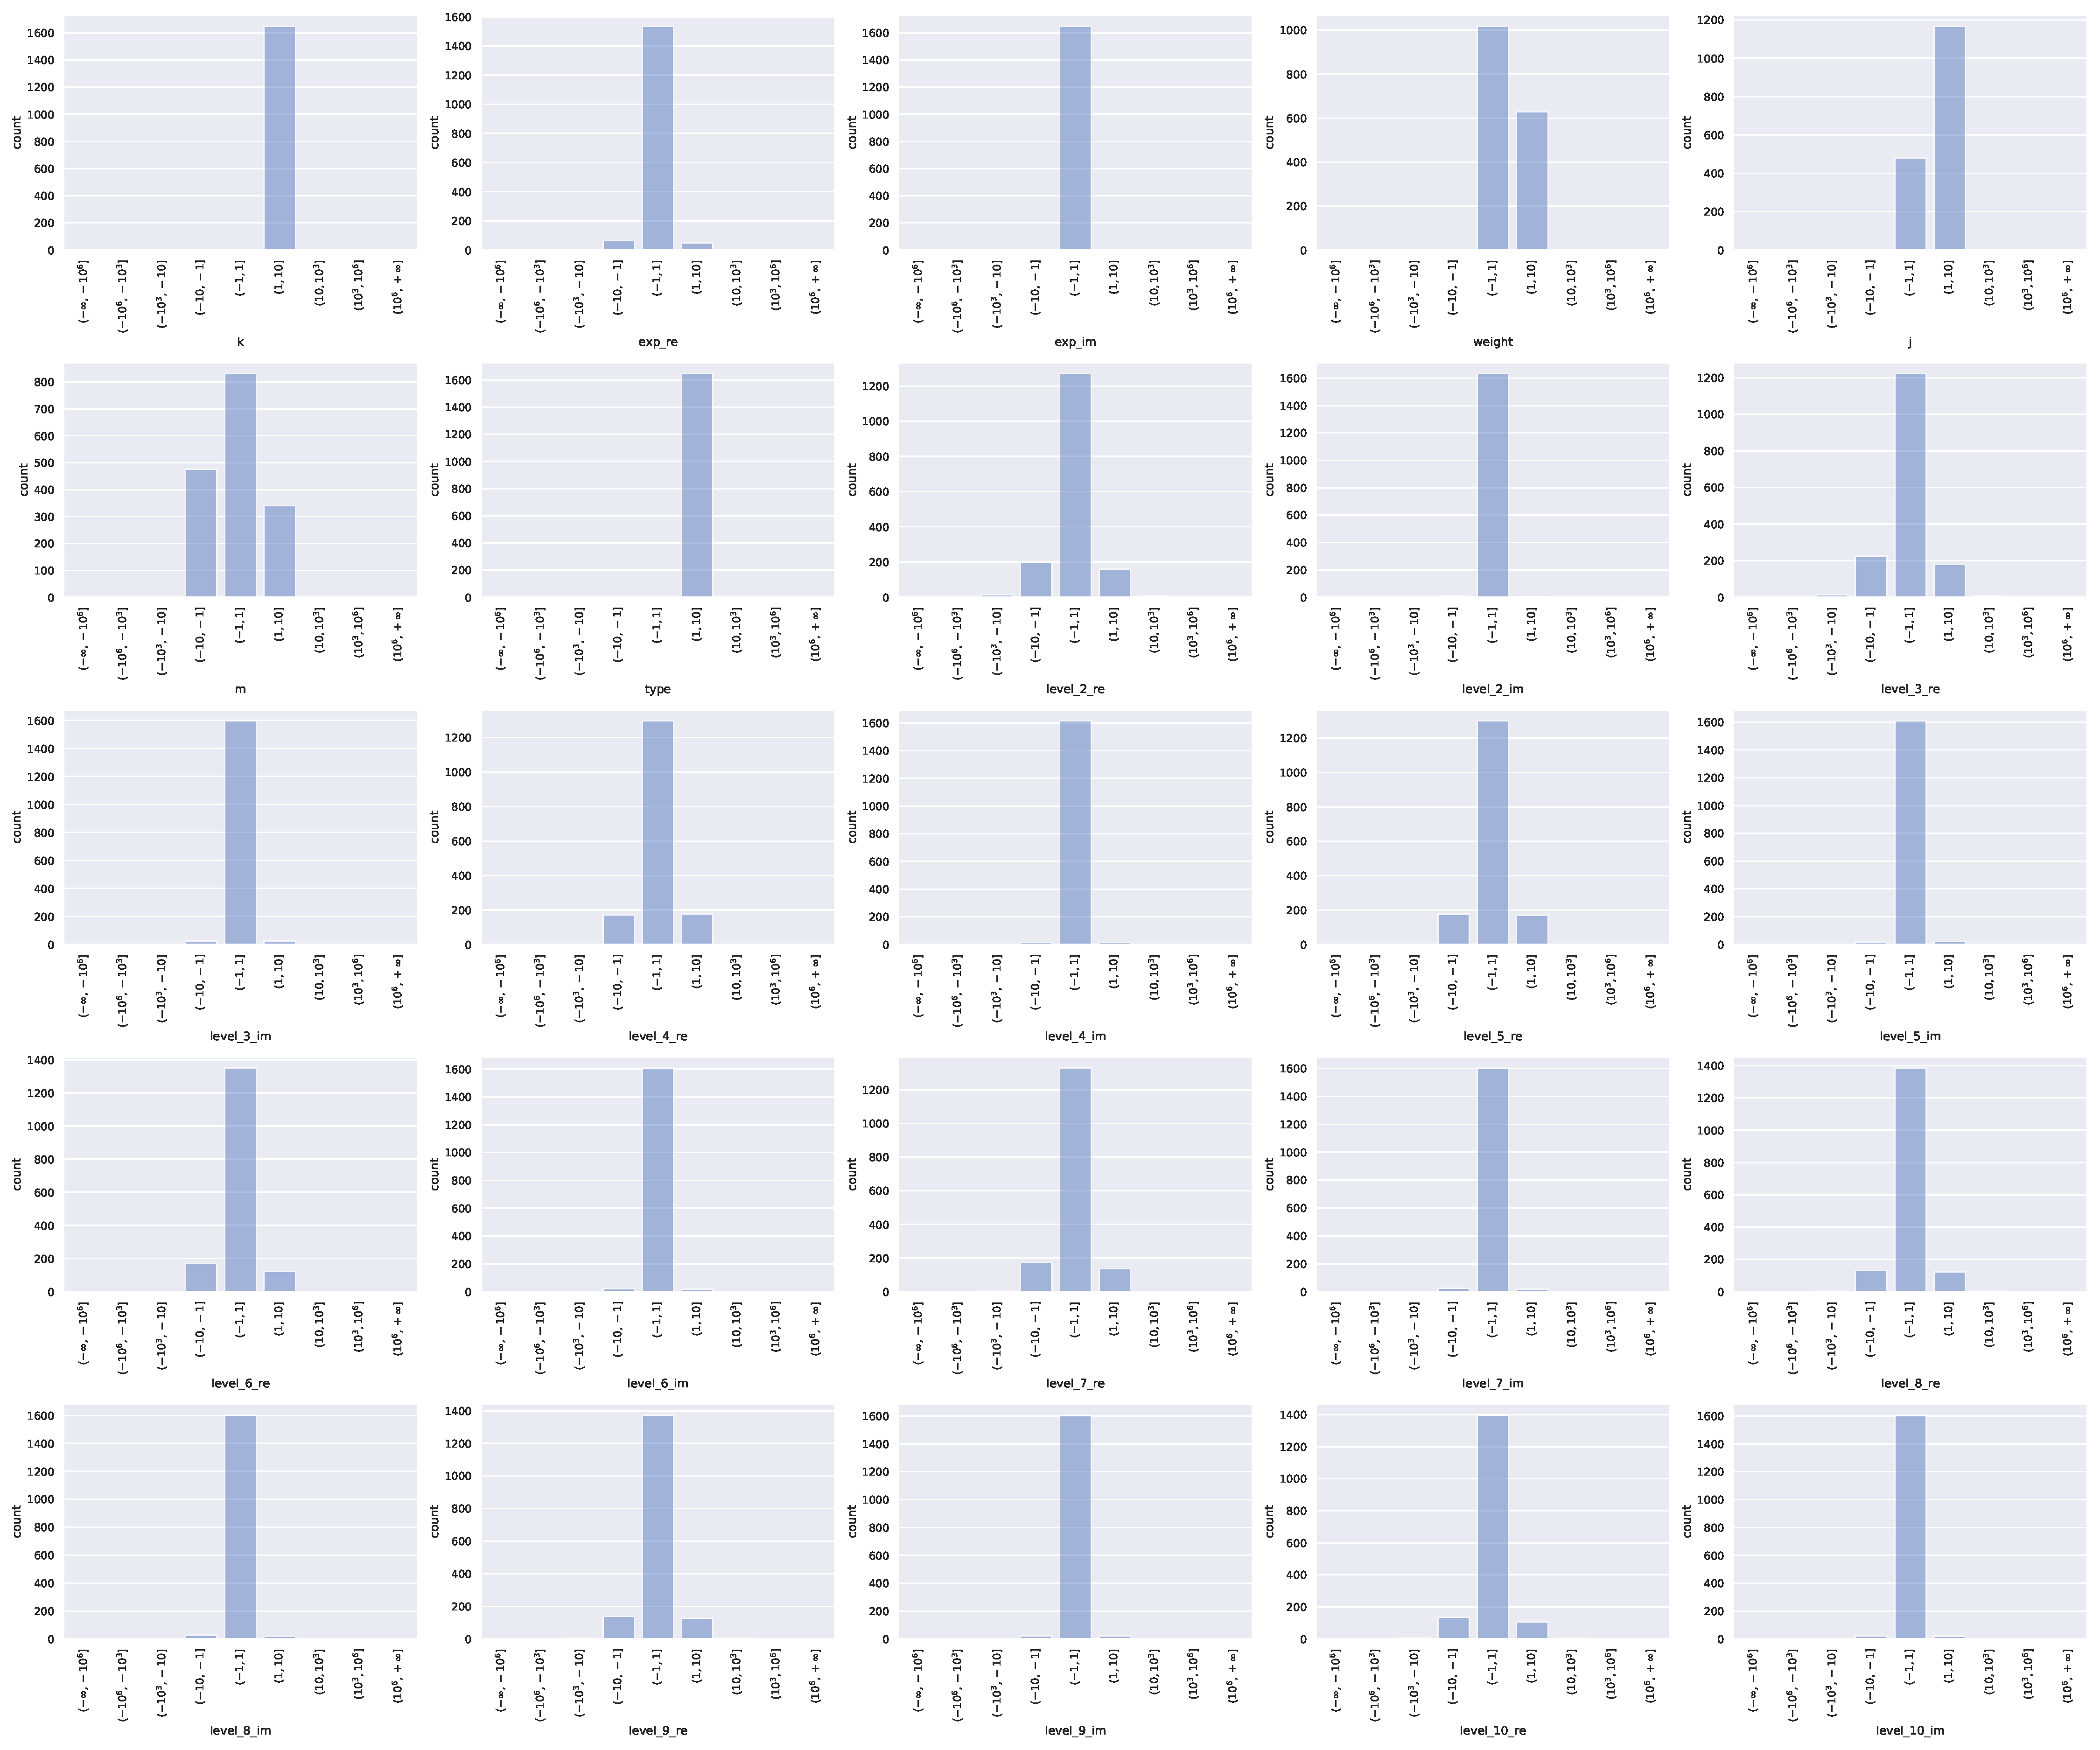
\includegraphics[width=0.6\textwidth]{img/var_counts}
  \caption{Distribution of the variables per order of magnitude.}
  \label{fig:wzw:counts}
\end{figure}


\subsubsection{Outliers Distribution}

Differently from the previous dataset the distribution of the variables is however more balanced (see \Cref{fig:wzw:counts}), even though the fraction of outliers is much larger than before.
However the large number of outliers is mainly due to the presence of non vanishing imaginary part in the truncation levels: only a small number of them is not a real number, thus the average of the imaginary part is narrowly peaked at 0 and any non vanishing contributions is an outlier (see \Cref{fig:wzw:outliers}).

\begin{figure}[htbp]
  \centering
  \begin{subfigure}{0.45\textwidth}
    \centering
    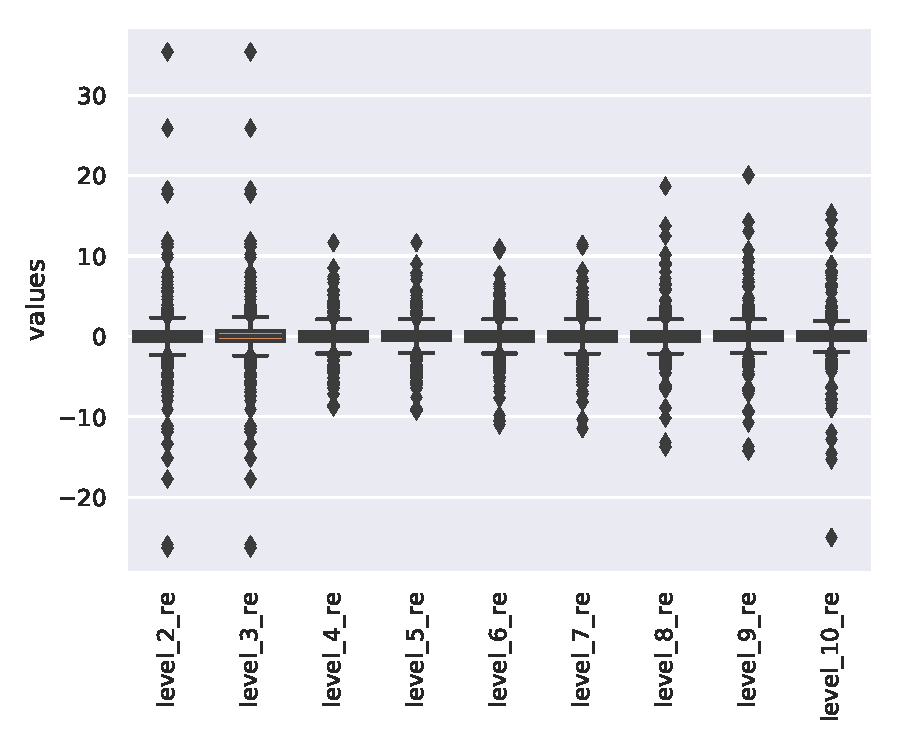
\includegraphics[width=\linewidth]{img/var_box_re}
    \caption{Real part.}
  \end{subfigure}
  \begin{subfigure}{0.45\textwidth}
    \centering
    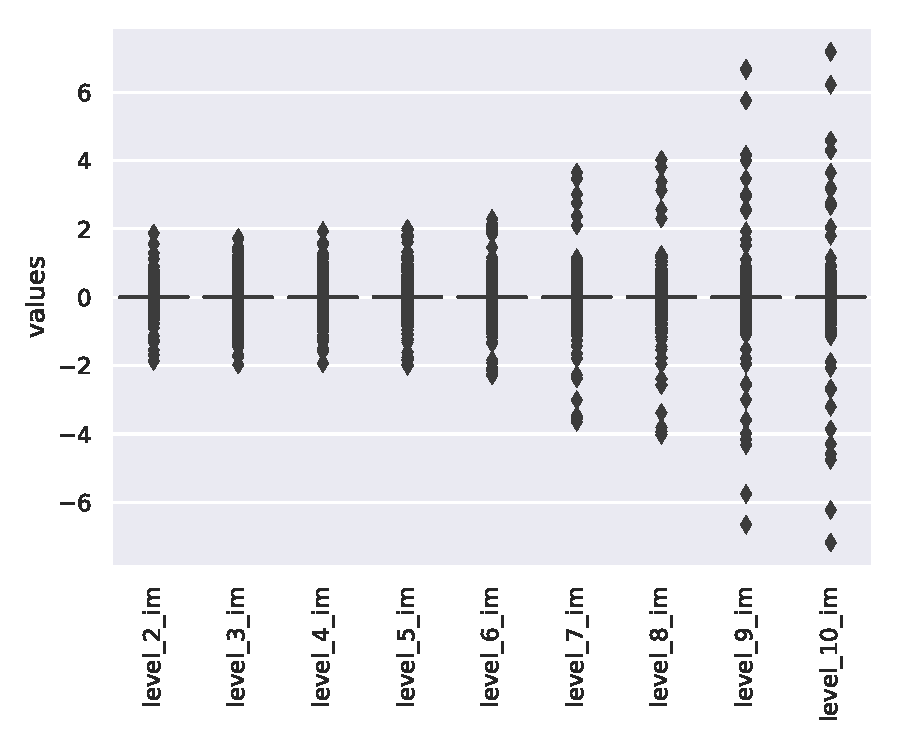
\includegraphics[width=\linewidth]{img/var_box_im}
    \caption{Imaginary part.}
  \end{subfigure}
  \caption{Outlier distribution.}
  \label{fig:wzw:outliers}
\end{figure}

As in the previous dataset there are however strong relations between the data which have been summarised in \Cref{tab:wzw:quantum}.
In particular we have:
\begin{itemize}
  \item \texttt{weight} $\ge 1.0$ and \texttt{type} $= 4$ and \texttt{k} $\in \lbrace 2, 3 \rbrace$ $\Rightarrow$ \texttt{weight} $= 1$ and \texttt{j} $= 0$ and \texttt{m} $= 0$,

  \item \texttt{weight} $\ge 1.0$ and \texttt{type} $= 4$ and \texttt{k} $= 4$ $\Rightarrow$ \texttt{weight} $= 1$,

  \item \texttt{type} $= 2$ $\Rightarrow$ \texttt{weight} $= 0$ and \texttt{j} $= 0$ and \texttt{m} $= 0$.
\end{itemize}

\begin{table}[htbp]
  \centering
  %\resizebox{\textwidth}{!}{%
  \begin{tabular}{@{}ccccccccc@{}}
  \toprule
                             &                    &            & \multicolumn{2}{c}{\textbf{weight}} & \multicolumn{2}{c}{\textbf{j}} & \multicolumn{2}{c}{\textbf{m}} \\
  \textbf{weight}            & \textbf{type}      & \textbf{k} & \textit{mean}     & \textit{var}    & \textit{mean}  & \textit{var}  & \textit{mean}  & \textit{var}  \\ \midrule
  \multirow{7}{*}{$\ge 1.0$} & \multirow{7}{*}{4} & 2          & 1.00              & 0.000           & 0.00           & 0.00          & 0.0            & 0.00          \\
                             &                    & 3          & 1.00              & 0.000           & 0.00           & 0.00          & 0.0            & 0.00          \\
                             &                    & 4          & 1.00              & 0.000           & 1.35           & 0.90          & 0.0            & 1.39          \\
                             &                    & 5          & 1.18              & 0.013           & 1.76           & 1.32          & 0.0            & 2.10          \\
                             &                    & 6          & 1.26              & 0.048           & 2.35           & 1.05          & 0.0            & 3.00          \\
                             &                    & 7          & 1.47              & 0.076           & 2.79           & 1.38          & 0.0            & 4.01          \\
                             &                    & 8          & 1.57              & 0.130           & 3.21           & 1.21          & 0.0            & 4.93          \\
  \midrule
  \multirow{14}{*}{$< 1.0$}  & \multirow{7}{*}{2} & 2          & 0.00              & 0.000           & 0.00           & 0.00          & 0.0            & 0.00          \\
                             &                    & 3          & 0.00              & 0.000           & 0.00           & 0.00          & 0.0            & 0.00          \\
                             &                    & 4          & 0.00              & 0.000           & 0.00           & 0.00          & 0.0            & 0.00          \\
                             &                    & 5          & 0.00              & 0.000           & 0.00           & 0.00          & 0.0            & 0.00          \\
                             &                    & 6          & 0.00              & 0.000           & 0.00           & 0.00          & 0.0            & 0.00          \\
                             &                    & 7          & 0.00              & 0.000           & 0.00           & 0.00          & 0.0            & 0.00          \\
                             &                    & 8          & 0.00              & 0.000           & 0.00           & 0.00          & 0.0            & 0.00          \\
  \cmidrule(l){2-9}
                             & \multirow{7}{*}{4} & 2          & 0.31              & 0.047           & 0.67           & 0.17          & 0.0            & 0.50          \\
                             &                    & 3          & 0.45              & 0.083           & 1.00           & 0.28          & 0.0            & 0.83          \\
                             &                    & 4          & 0.38              & 0.053           & 1.00           & 0.26          & 0.0            & 0.77          \\
                             &                    & 5          & 0.50              & 0.090           & 1.33           & 0.39          & 0.0            & 1.18          \\
                             &                    & 6          & 0.44              & 0.071           & 1.33           & 0.40          & 0.0            & 1.14          \\
                             &                    & 7          & 0.56              & 0.108           & 1.67           & 0.56          & 0.0            & 1.67          \\
                             &                    & 8          & 0.50              & 0.089           & 1.66           & 0.56          & 0.0            & 1.64          \\ \bottomrule
  \end{tabular}%
  %}
  \caption{Relations between the weight and type variables, and other quantum numbers.}
  \label{tab:wzw:quantum}
\end{table}


\subsubsection{Correlation Matrix}

Finally we show the correlation matrix of the features in \Cref{fig:wzw:corr}.
From the correlations it is no longer recognisable an oscillating behaviour as in the previous case.
However we notice that real and imaginary parts are separately highly correlated features (though they are completely non correlated between them).
Differently from the previous case the \texttt{weight} variable is poorly correlated, apart from the previously mentioned relation with \texttt{j}.

\begin{figure}[htbp]
  \centering
  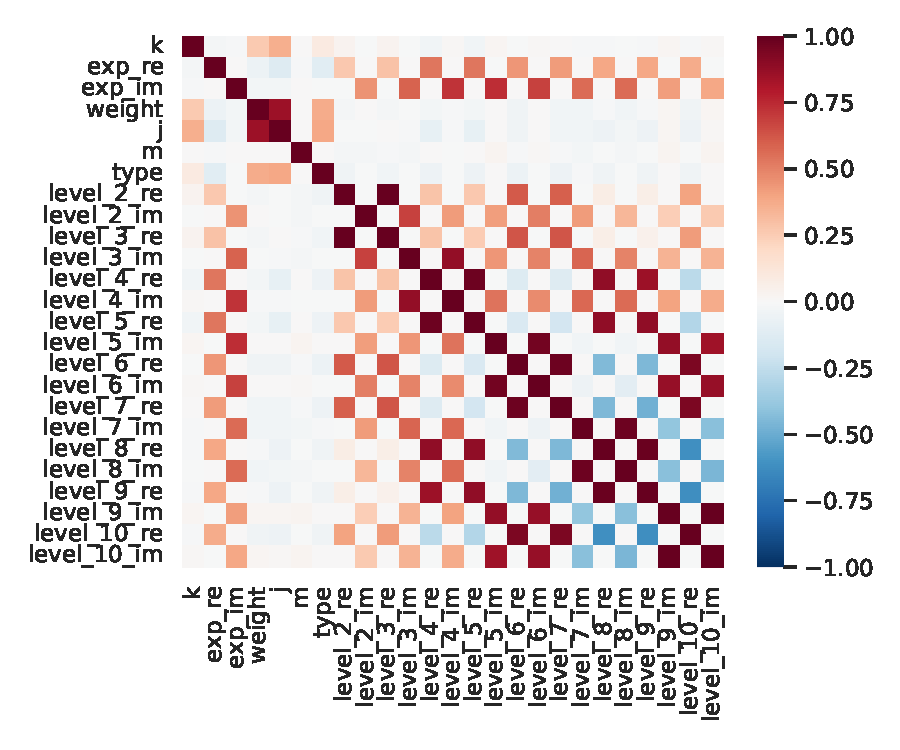
\includegraphics[width=0.6\textwidth]{img/wzw_corr_mat}
  \caption{Correlation matrix of the \wzw model.}
  \label{fig:wzw:corr}
\end{figure}


\subsubsection{Principal Components Analysis}

As in the previous case, we also analyse the principal components of the truncation levels.
We perform the analysis in two separate ways: in the first we consider the whole group of truncation levels and robustly scale them against outliers (using the \texttt{RobustScaler} class in \texttt{Scikit-learn}), in the second we separate real and imaginary parts, standardise the first (using the \texttt{StandardScaler} in \texttt{Scikit-learn}) and robustly scale the latter.
We then perform the same analysis as before.
As we see in \Cref{fig:wzw:svd}, in both cases a large part of the variance is already captures by one of the principal components (both the whole and separate datasets retain more than \SI{99}{\percent} of the variance with just one component).
It may therefore be possible to use the principal components to have a fixed input size for the algorithms and be compatible with other datasets.

\begin{figure}[htbp]
  \centering
  \begin{subfigure}{0.45\textwidth}
    \centering
    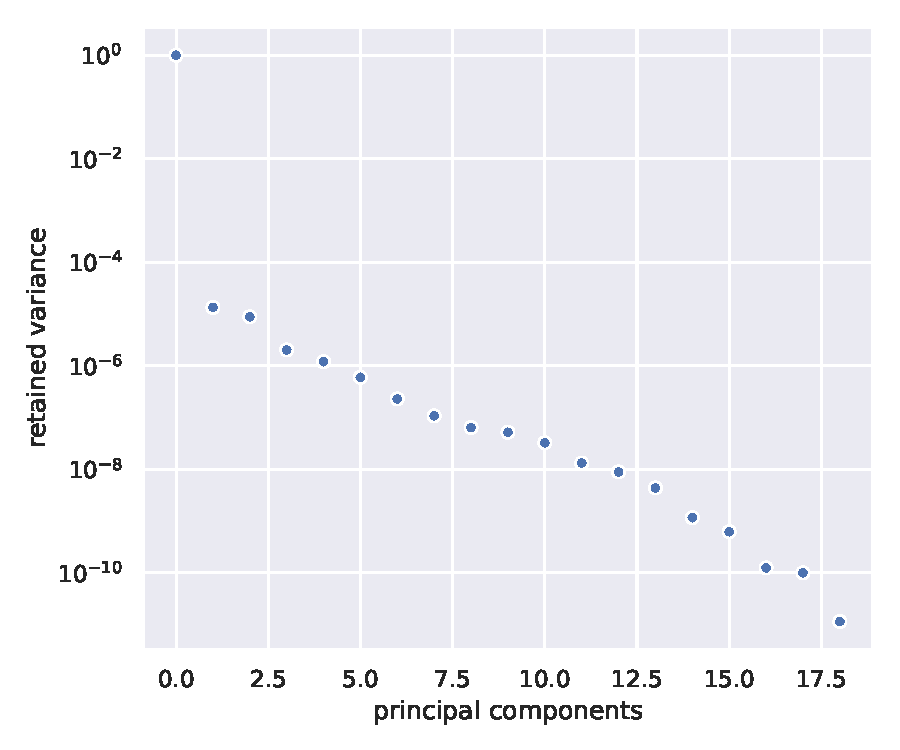
\includegraphics[width=\linewidth]{img/wzw_svd_tot}
    \caption{Whole dataset.}
  \end{subfigure}
  \begin{subfigure}{0.45\textwidth}
    \centering
    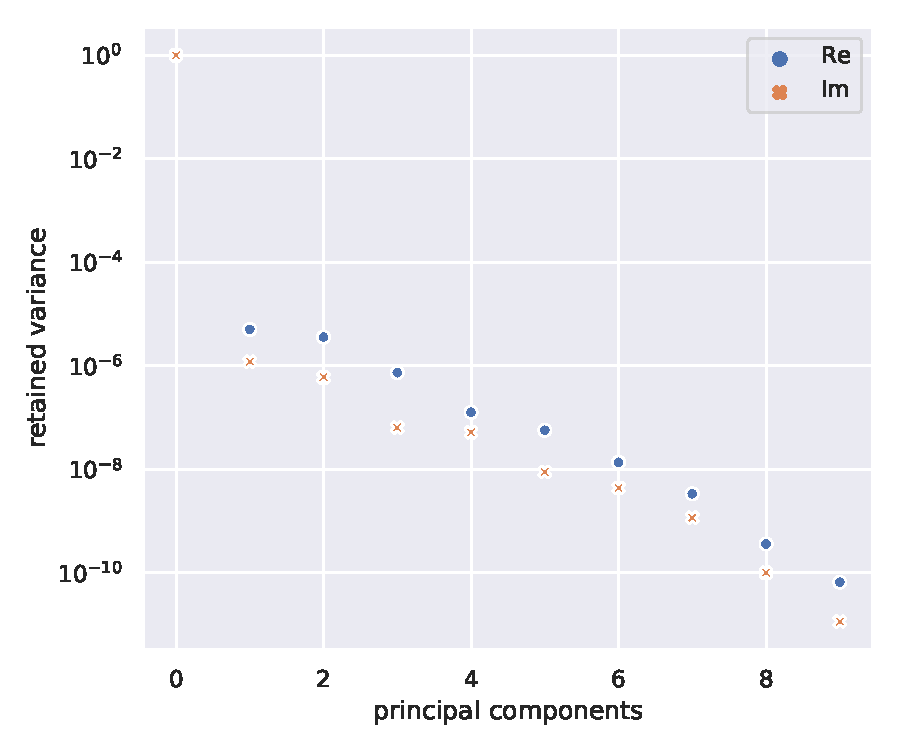
\includegraphics[width=\linewidth]{img/wzw_svd_sep}
    \caption{Separate dataset.}
  \end{subfigure}
  \caption{Principal components of the truncation levels.}
  \label{fig:wzw:svd}
\end{figure}


\subsection{Statistical Inference}

As for the previous case, using the \eda data we performed the \anova on the \wzw model using a simple linear regression.
For this we used \SI{80}{\percent} of the dataset for training and the rest as development set: since the data is already labelled, we do not need to separate the samples according to the \texttt{solutions} variable.
However in this case we will keep all the variables present in the dataset and perform the regression predicting both the real and imaginary parts of \texttt{exp} simultaneously.

With 313 \dof we reached a \mse of 0.06 with a \ci $\left[0.0, 0.07\right]$ and $\rr = 0.83$ (both are better than the previous dataset signalling that features and labels may be more correlated in this case).

\begin{table}[htbp]
  \centering
  \resizebox{\textwidth}{!}{%
  \begin{tabular}{@{}ccccccccc@{}}
  \toprule
                         & \textbf{coeff.\ -- Re}
                         & \textbf{coeff.\ -- Im}
                         & \textbf{std.\ err.\ -- Re}
                         & \textbf{std.\ err.\ -- Im}
                         & \textbf{t -- Re}
                         & \textbf{t -- Im}
                         & \textbf{p-value ($t_{obs} \ge \abs{t}$) -- Re}
                         & \textbf{p-value ($t_{obs} \ge \abs{t}$) -- Im} \\
  \midrule
  \texttt{k}             & 0.003  & -0.005  & 0.015 & 0.002   & 0.176    & -2.977   & 0.861  & 0.003  \\
  \texttt{weight}        & 0.05   & -0.005  & 0.03  & 0.004   & 1.520    & -1.361   & 0.130  & 0.175  \\
  \texttt{j}             & -0.033 & 0.00035 & 0.015 & 0.0017  & -2.263   & 0.211    & 0.024  & 0.833  \\
  \texttt{m}             & 0.000  & 0.0003  & 0.013 & 0.0014  & 0.075    & 0.230    & 0.940  & 0.818  \\
  \texttt{type}          & 0.00   & 0.010   & 0.04  & 0.0047  & 0.058    & 2.234    & 0.954  & 0.026  \\
  \texttt{Re(level 2)}   & 0.329  & 0.0088  & 0.006 & 0.0007  & 51.791   & 12.163   & 0.000  & 0.000  \\
  \texttt{Im(level 2)}   & 0.02   & -0.034  & 0.09  & 0.011   & 0.265    & -3.271   & 0.791  & 0.001  \\
  \texttt{Re(level 3)}   & -0.349 & -0.0086 & 0.006 & 0.0007  & -55.653  & -12.120  & 0.000  & 0.000  \\
  \texttt{Im(level 3)}   & -0.07  & -0.064  & 0.05  & 0.006   & -1.242   & -10.764  & 0.215  & 0.000  \\
  \texttt{Re(level 4)}   & -0.516 & 0.0145  & 0.015 & 0.0017  & -35.415  & 8.785    & 0.000  & 0.000  \\
  \texttt{Im(level 4)}   & 0.11   & 0.062   & 0.06  & 0.006   & 1.890    & 9.801    & 0.060  & 0.000  \\
  \texttt{Re(level 5)}   & -0.036 & -0.0175 & 0.014 & 0.0016  & -2.519   & -10.871  & 0.012  & 0.000  \\
  \texttt{Im(level 5)}   & -0.10  & -1.507  & 0.05  & 0.006   & -2.019   & -267.397 & 0.044  & 0.000  \\
  \texttt{Re(level 6)}   & -4.931 & -0.0256 & 0.014 & 0.0016  & -340.537 & -15.605  & 0.000  & 0.000  \\
  \texttt{Im(level 6)}   & 0.15   & 1.939   & 0.05  & 0.006   & 2.960    & 346.379  & 0.003  & 0.000  \\
  \texttt{Re(level 7)}   & 4.539  & 0.0262  & 0.014 & 0.0016  & 328.362  & 16.776   & 0.000  & 0.000  \\
  \texttt{Im(level 7)}   & -0.00  & -3.980  & 0.04  & 0.005   & -0.132   & -807.934 & 0.895  & 0.000  \\
  \texttt{Re(level 8)}   & -3.71  & -0.0383 & 0.013 & 0.0015  & -279.284 & -25.439  & 0.000  & 0.000  \\
  \texttt{Im(level 8)}   & -0.04  & 4.444   & 0.04  & 0.005   & -0.991   & 960.701  & 0.322  & 0.000  \\
  \texttt{Re(level 9)}   & 4.684  & 0.0406  & 0.013 & 0.0014  & 367.810  & 28.150   & 0.000  & 0.000  \\
  \texttt{Im(level 9)}   & 0.08   & -2.587  & 0.03  & 0.003   & 2.756    & -775.714 & 0.006  & 0.000  \\
  \texttt{Re(level 10)}  & 0.874  & 0.0009  & 0.012 & 0.0013  & 75.406   & 0.693    & 0.000  & 0.489  \\
  \texttt{Im(level 10)}  & -0.14  & 2.687   & 0.03  & 0.003   & -4.800   & 840.827  & 0.000  & 0.000  \\                                                  
  \bottomrule
  \end{tabular}%
  }
  \caption{Results of the \anova on the linear model.}
  \label{tab:wzw:anova}
\end{table}

In \Cref{tab:wzw:anova} we show the results of the analysis: we show the choice of the coefficients and their statistics in separate columns for the real and imaginary parts of \texttt{exp}).
Differently from the previous case the data is a bit more complex and in some cases it shows that we could actually drop some of the variables.
For instance we will certainly drop \texttt{k} which does not seem to influence the final result (its p-value is very high).
Curiously enough, it seems that in order to predict $\Re(exp)$ we could just use the real parts of the variables in the dataset, while the situation for $\Im(exp)$ requires the contributions of both real and imaginary parts of the input features.


\subsection{Model Dependent Deep Learning Analysis}


As a prosecution of the exploratory analysis we also performed a prediction analysis using the same ANN model used for the previous dataset.
The necessary modifications however concern the input shape of the architecture (here we have more input variables) and the output layer: we are interested in predicting both real and imaginary parts of the output at the same time.
This in turn will not be necessary for the aggregate analysis but it might be worth noting the results.

For the learning model we split the dataset into \SI{80}{\percent} for training, \SI{10}{\percent} for validation and the remaining \SI{10}{\percent} as a test set.
In general the ANN model behaved extremely well in the training and validation folds, while it performed poorly in the test set: the \rr score for both $\Re(exp)$ and $\Im(exp)$ dropped respectively to \num{0.66} and \num{0.30} in the test set while it was above \num{0.94} in both cases for the training and validation folds.\footnotemark{}
\footnotetext{%
  As a consequence also the \mse plummeted in the test set.
}
This however seems to be entirely due to a small number of samples in the test set which drove away the \mse and the \rr score with respect to the validation and training sets.
In \Cref{fig:wzw:preds} we can clearly see the sample (the same between real and imaginary parts) spoiling the result.

\begin{figure}[htbp]
  \centering
  \begin{subfigure}{0.45\textwidth}
    \centering
    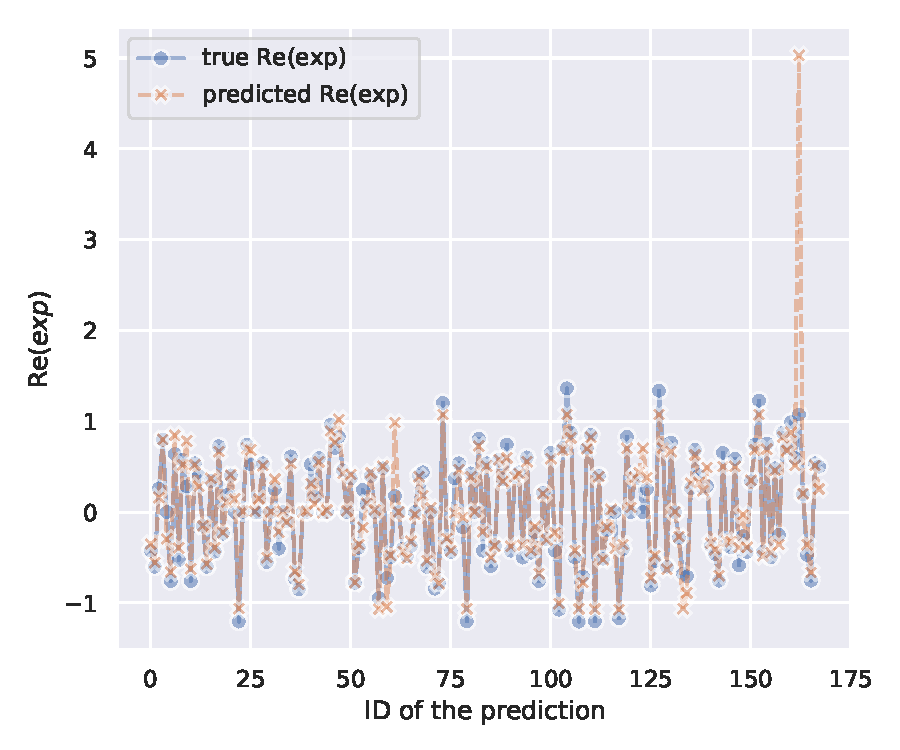
\includegraphics[width=\linewidth]{img/ann_model_test_re_lineplot}
    \caption{Real part.}
  \end{subfigure}
  \begin{subfigure}{0.45\textwidth}
    \centering
    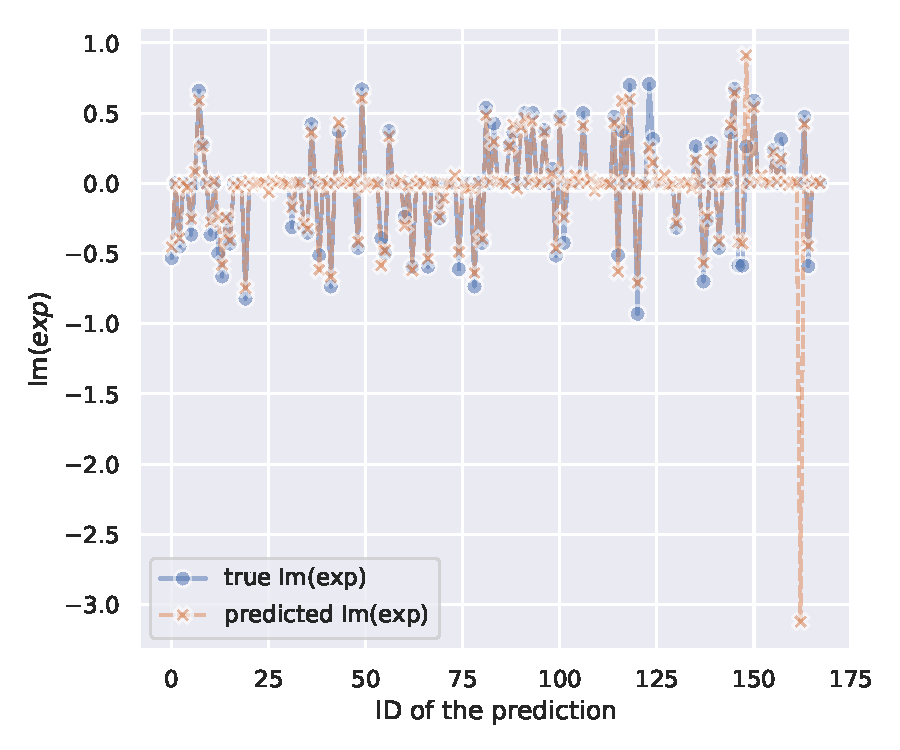
\includegraphics[width=\linewidth]{img/ann_model_test_im_lineplot}
    \caption{Imaginary part.}
  \end{subfigure}
  \caption{Predictions and true values of the \texttt{exp} label.}
  \label{fig:wzw:preds}
\end{figure}



\section{Aggregate Analysis}
\subsection{Preparation of the Input}

In this section we focus on predicting both real and imaginary parts of the \texttt{exp} label using both the lumps and the \wzw datasets together: the idea is to have a model independent architecture able to make predictions without knowledge of the underlying physical model.

The datasets are however defined differently and many variables differ in the two physical models.
We start from the tidy datasets which have been prepared for the separate analysis in the previous sections.

We will proceed as follows, before merging the datasets:
\begin{itemize}
  \item we define an effective weight $\hat{h}$ in the \wzw model such that $\hat{h} = \abs{h \cdot m}$, where $h$ is the value of the \texttt{weight} variable in the dataset and $m$ is one of the quantum numbers associated with the \SU{2} representation,\footnotemark{}
    \footnotetext{%
      The idea is to have an engineered feature which combines \texttt{k}, \texttt{j} and \texttt{m} in the same range as the \texttt{weight} variable in the lumps dataset.
    }
  \item we transform the columns in the lumps dataset to account for the imaginary parts of the truncation levels (in this dataset they will be identically vanishing),
  \item we compute the PCA of the truncation levels in both datasets, keeping 10 components each to maximise the retained variance,
  \item in the lumps dataset we then select the \texttt{weight}, \texttt{type} and the PCA variables,
  \item in the \wzw dataset we select the effective weight, \texttt{type} and the PCA variables,
  \item we \emph{outer join} the datasets on the \texttt{weight} and \texttt{type} variables.
\end{itemize}
We finally have a new dataset containing 12 features and 2 labels (i.e.\ $\Re(exp)$ and $\Im(exp)$), and 2379 samples.


\subsection{Validation Strategy}

For the analysis we keep \SI{80}{\percent} of the samples for training, \SI{10}{\percent} for validation and \SI{10}{\percent} as a test set as we did before for the two separate datasets.
In this case the datasets can be freely shuffled since all the information on the model is already encoded in the variables.

Before passing the input to the algorithms we scale it using the \texttt{StandardScaler} class in \texttt{Scikit-learn} in order to standardise the features and simplify the learning process.
The labels are not scaled, thus the predictions are directly comparable with the ground truth values.

We focus on predicting both $\Re(exp)$ and $\Im(exp)$ at the same time with a single model.
We will use, as a comparison, the SVM with the Gaussian kernel and an ANN model.
However, since the first cannot naturally account for two outputs, we use the \texttt{MultiOutputRegressor} class in \texttt{Scikit-learn} which automatically uses the same estimator to predict separately both labels.

We will finally provide also the predictions on the double lumps using the trained models to check the ability to generalise to other datasets.


\subsection{Support Vector Machines}

\subsubsection{Training}

The model used for training is a single architecture to predict both real and imaginary parts of \texttt{exp}.
We do not perform any automatic optimisation since the interface with the \emph{Scikit-optimize} Bayes cycle does not allow to predict two labels at the same time.
Moreover hyperparameters chosen for predicting $\Re(exp)$ are in principle different from those used to predict $\Im(exp)$.
We manually choose $C = 10^5$, $\epsilon= 0.1$ and $\gamma = 0.1$ (respectively reffering to the penalty assigned to distant samples, the \emph{no penalty} rigid boundary, and the width of the Gaussian kernel).


\subsubsection{Results}

Results on the test fold are summarised in \Cref{tab:agg:svr_met}.
Even though the algorithm performed well on the validation set ($\mse = 0.09$ for $\Re(exp)$ and $\mse = 0.03$ for $\Im(exp)$), the results on the generalisation set are one order of magnitude larger.
Even though it may be difficult to isolate the cause, it seems the worst result is mainly due to very few samples whose predictions is heavily influecing the bad result, as shown in \Cref{fig:agg:svr_pred}.
We will therefore need to check these predictions, since the algorithm seems to perform quite well otherwise, as the residual plot shows in \Cref{fig:agg:svr_res_plot}.

\begin{table}[htbp]
  \centering
  %\resizebox{\textwidth}{!}{%
  \begin{tabular}{@{}ccccc@{}}
  \toprule
             & \dof & \mse & \mae & \rr   \\
  \midrule
  $\Re(exp)$ & 226  & 0.3  & 0.15 & 0.36  \\
  $\Im(exp)$ & 226  & 0.3  & 0.11 & -3.4  \\
  \bottomrule
  \end{tabular}%
  %}
  \caption{Summary of the metrics of the \emph{r-SVR} on the test set.}
  \label{tab:agg:svr_met}
\end{table}

\begin{figure}[htbp]
  \centering
  \begin{subfigure}{0.45\textwidth}
    \centering
    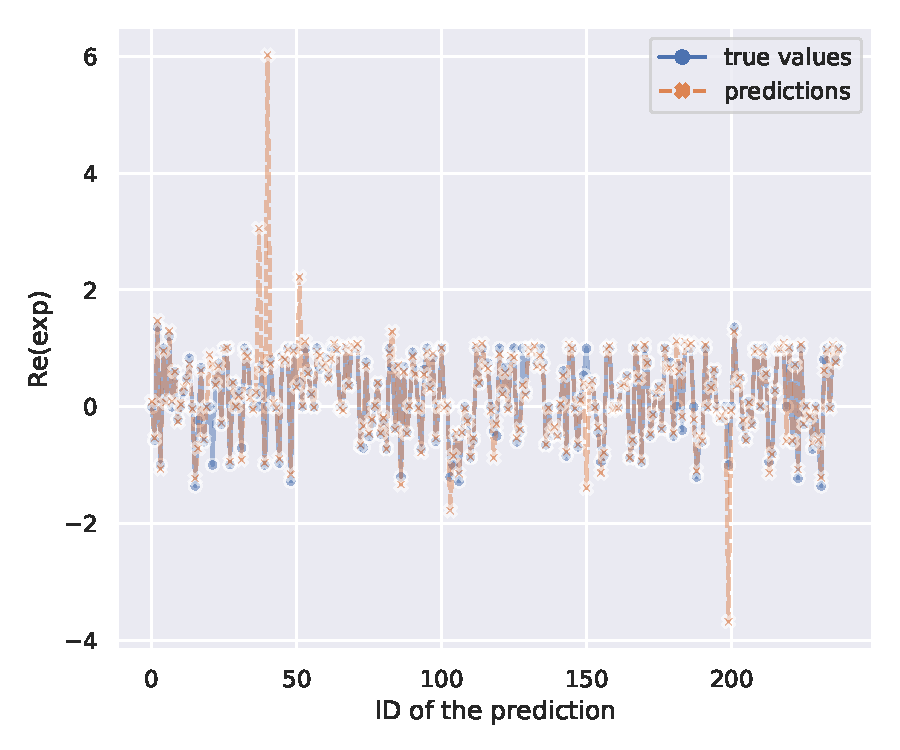
\includegraphics[width=\linewidth]{img/svr_test_exp_re_plot}
    \caption{Real part.}
  \end{subfigure}
  \begin{subfigure}{0.45\textwidth}
    \centering
    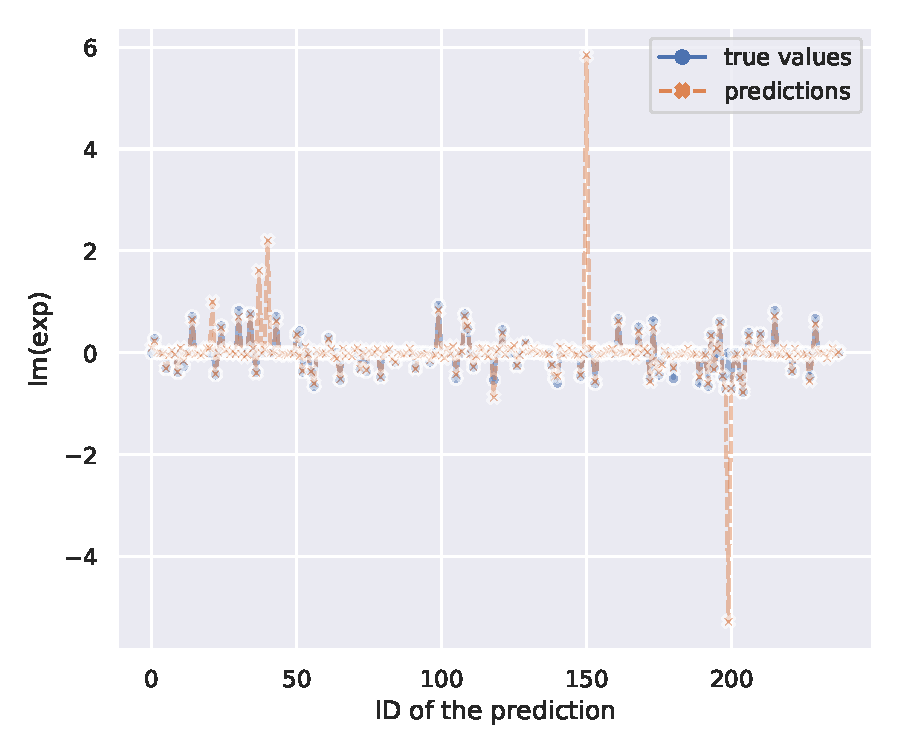
\includegraphics[width=\linewidth]{img/svr_test_exp_im_plot}
    \caption{Imaginary part.}
  \end{subfigure}
  \caption{Predictions and true values using the \emph{r-SVR} algorithm.}
  \label{fig:agg:svr_pred}
\end{figure}

\begin{figure}[htbp]
  \centering
  \begin{subfigure}{0.45\textwidth}
    \centering
    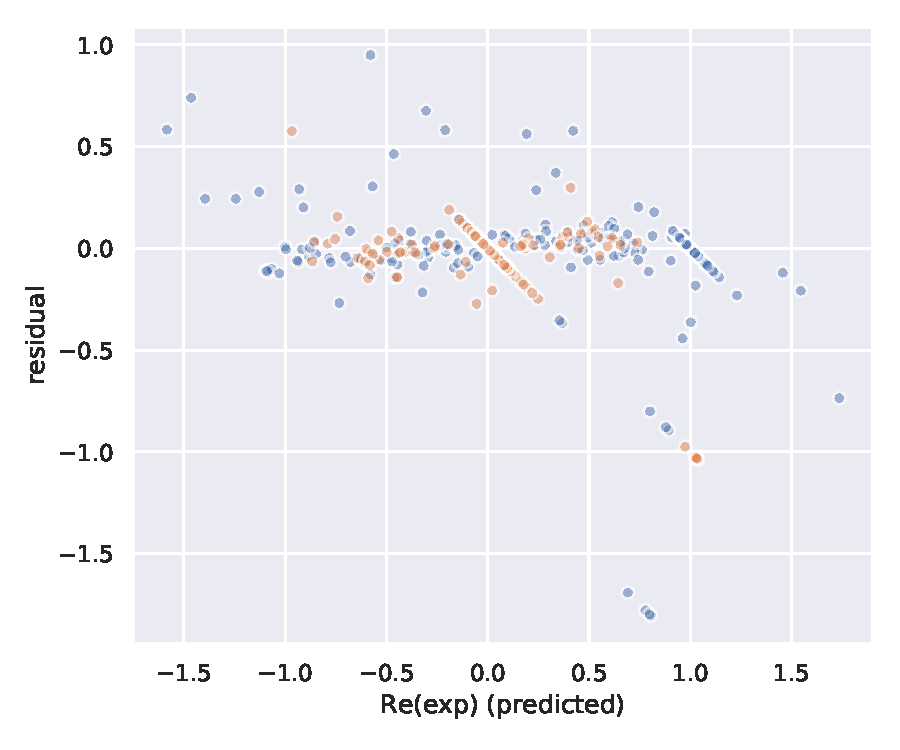
\includegraphics[width=\linewidth]{img/svr_val_res_plot}
    \caption{Validation set.}
  \end{subfigure}
  \begin{subfigure}{0.45\textwidth}
    \centering
    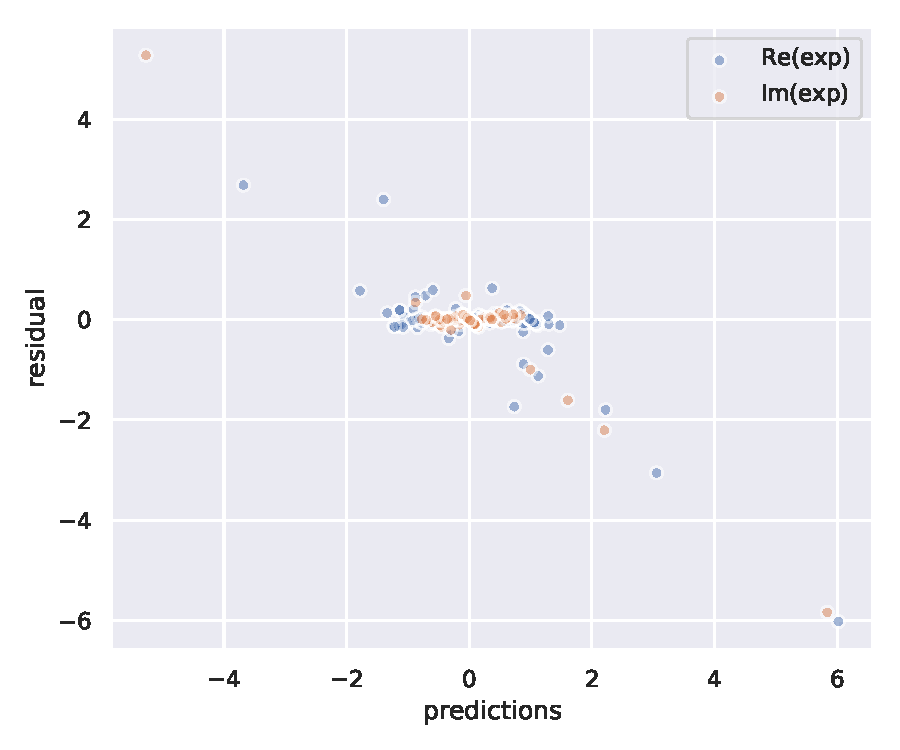
\includegraphics[width=\linewidth]{img/svr_test_res_plot}
    \caption{Test set.}
  \end{subfigure}
  \caption{Residual plot using the \emph{r-SVR}.}
  \label{fig:agg:svr_res_plot}
\end{figure}


\subsection{Artificial Neural Network}

\subsubsection{Model}

The model we use for training is a simple fully connected network (summarised in \Cref{tab:agg:keras_summary}).
The architecture is made of 4 hidden layers with \numlist{30;30;10;10} units each and dropout layers (with rate \num{0.05}) after the first two hidden layers (see \Cref{fig:agg:arch}).
The addition of batch normalisation layers drastically increased the error, so we dropped them entirely in this implementation.

\begin{table}[htbp]
  \centering
  \begin{tabular}{@{}lcc@{}}
    \toprule
    \textbf{layer}           & \textbf{shape} & \textbf{parameters} \\
    \midrule
    \emph{input}             & (12,)          & 0                   \\
    \emph{fully connected}   & (30,)          & 390                 \\
    \emph{dropout}           & (30,)          & 0                   \\
    \emph{fully connected}   & (30,)          & 930                 \\
    \emph{dropout}           & (30,)          & 0                   \\
    \emph{fully connected}   & (10,)          & 310                 \\
    \emph{fully connected}   & (10,)          & 110                 \\
    $\Re(exp)$ (output)      & (1,)           & 11                  \\
    $\Im(exp)$ (output)      & (1,)           & 11                  \\
    \midrule
    \emph{Total parameters:}     & \num{1762}     &                 \\
    \emph{Trainable parameters:} & \num{1762}     &                 \\
    \bottomrule
  \end{tabular}
  \caption{Summary of the network.}
  \label{tab:agg:keras_summary}
\end{table}

\begin{figure}[htbp]
  \centering
  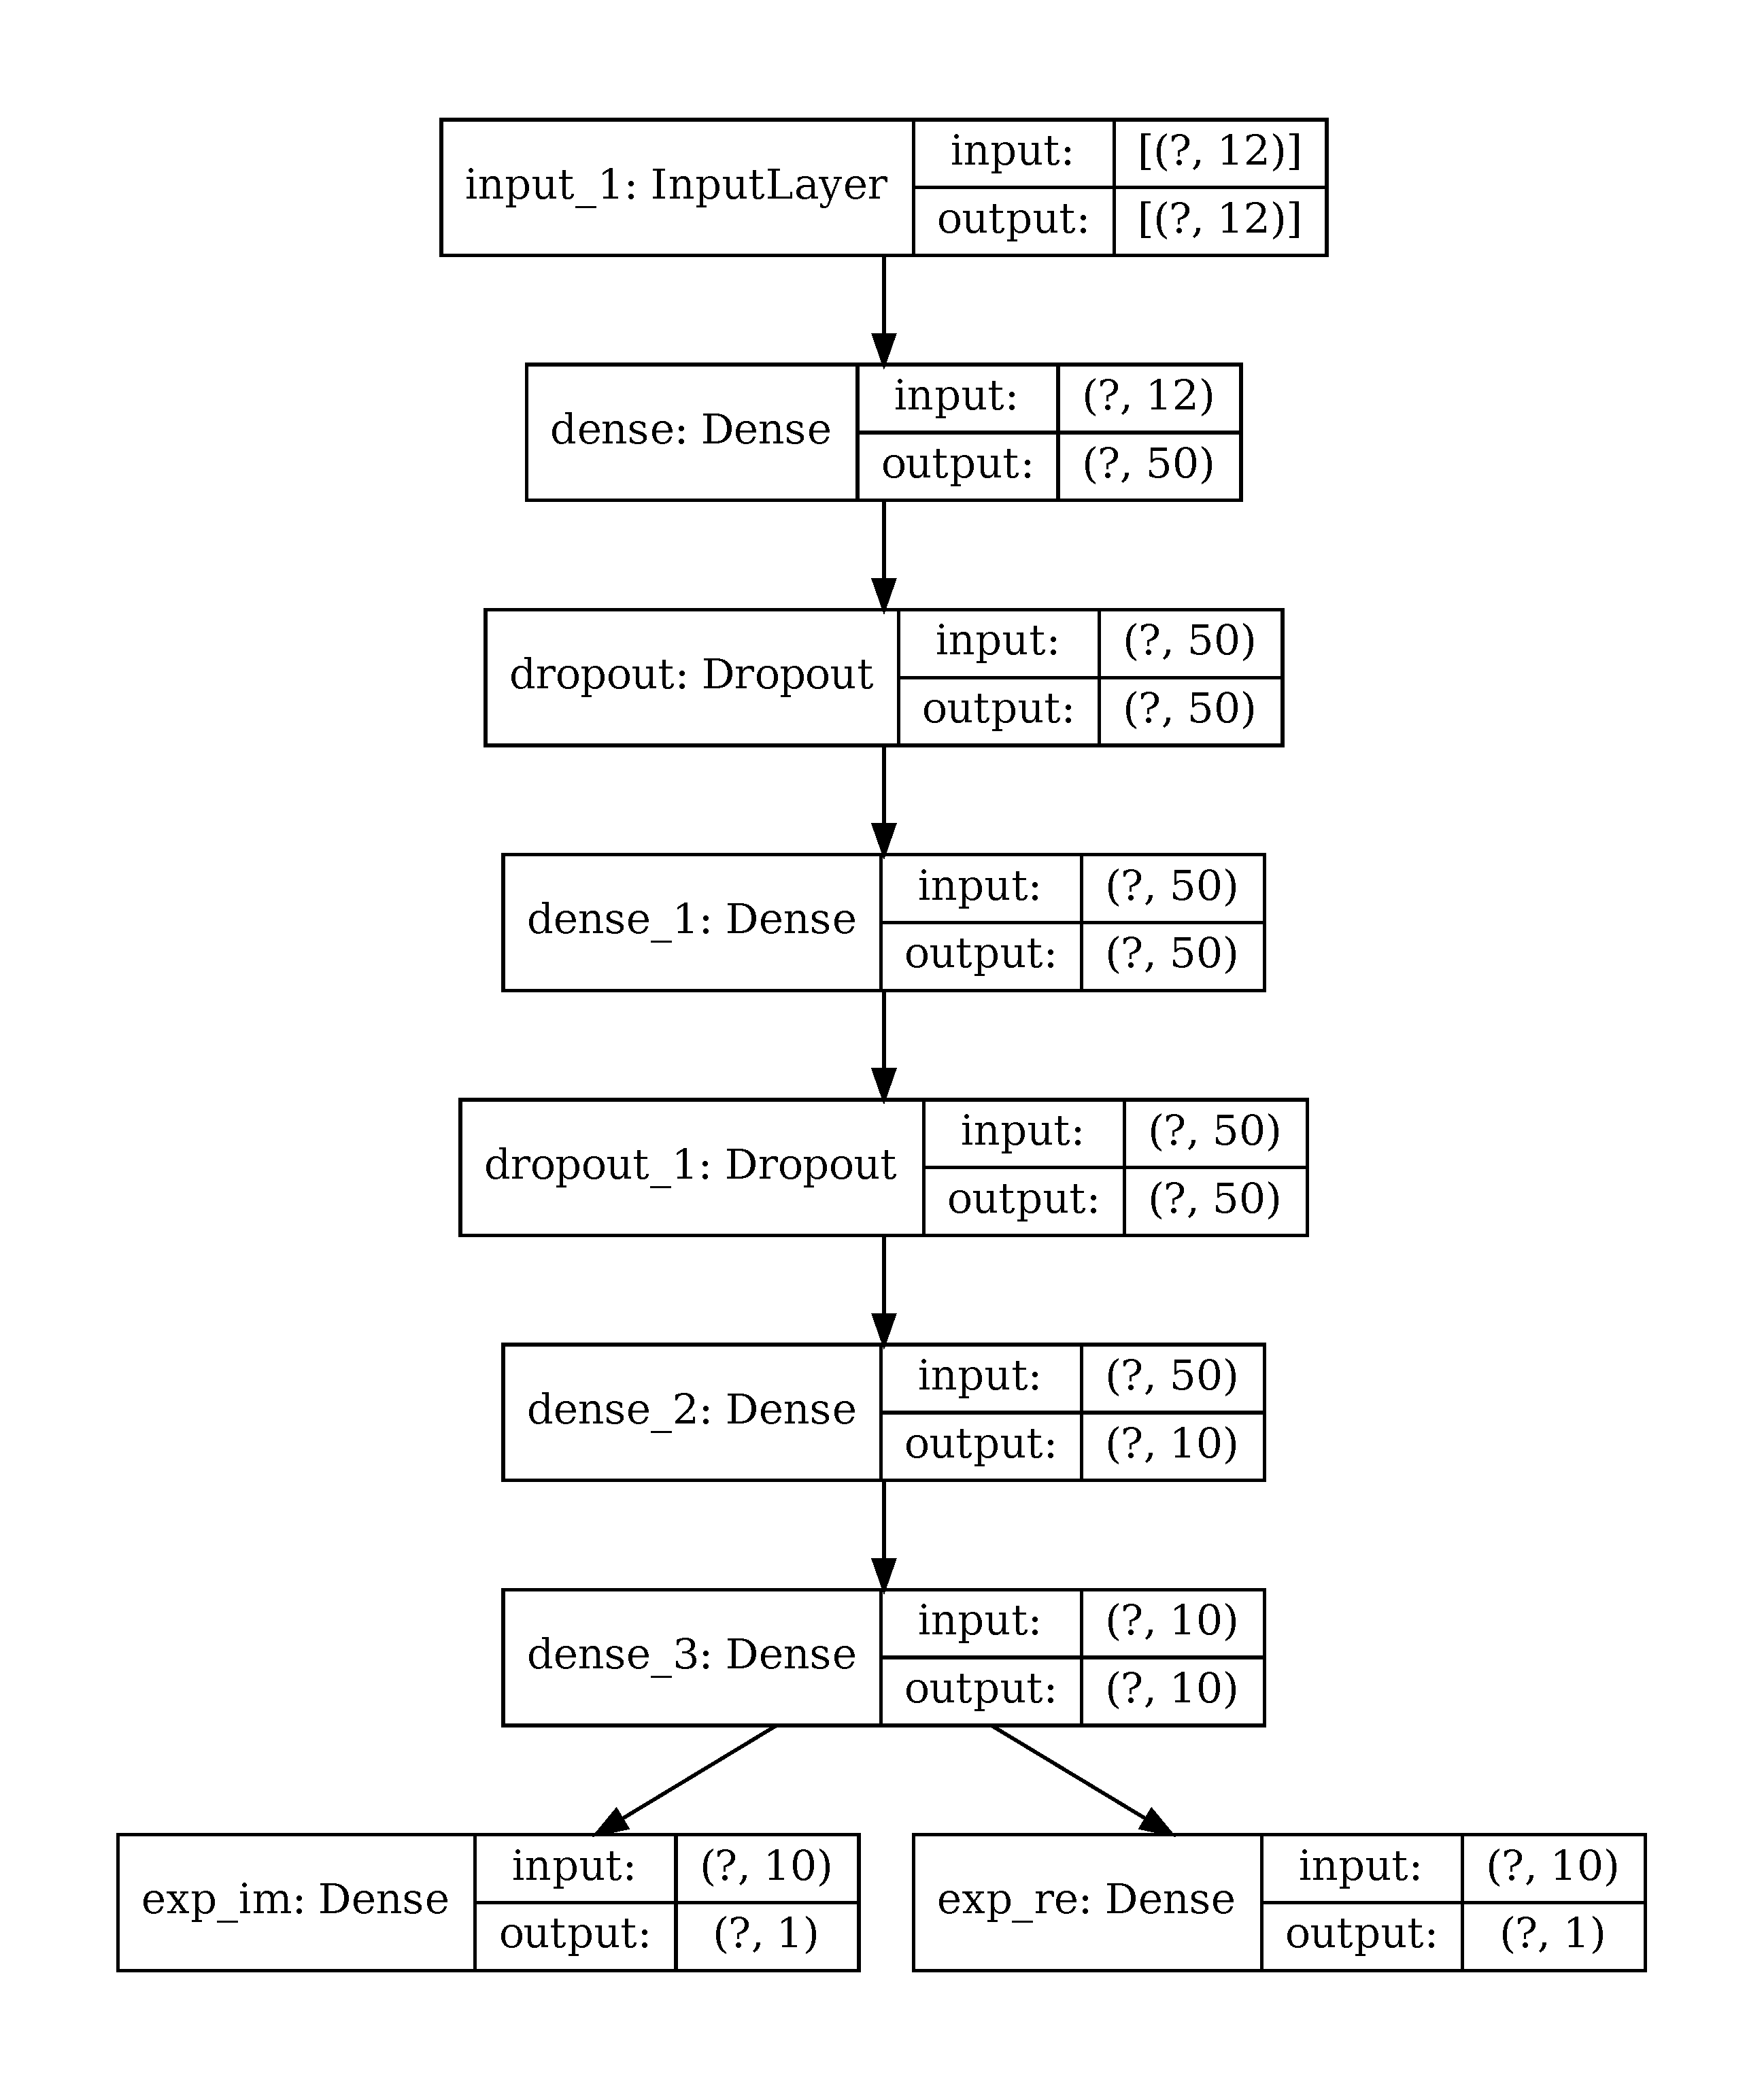
\includegraphics[width=0.6\textwidth]{img/ann_arch}
  \caption{Architecture of the ANN.}
  \label{fig:agg:arch}
\end{figure}


\subsubsection{Training}

For training we use the \mse as loss function and weigh it on the two output layers eavenly with \numlist{0.5;0.5} loss weights.\footnotemark{}
\footnotetext{%
  The loss function must be a scalar metric, thus the \mse in this case is separately computed on the output layers and then combined using the loss weights by multiplying each loss by its weight.
}
For gradient descent we use the \emph{Adam} optimiser with default values and initial learning rate of \num{0.001} and a mini batch size of 32.
The maximal number of epochs used for training is \num{20000} but it greatly exceeds what actually needed for good results.
In fact we also implement a callback to early stop the training after 1000 epochs without improvement of the loss function on the validation data.
We finally add a callback to reduce the learning rate by a step factor of \num{0.3} after 750 epochs without improvement on the validation loss.

The loss function and the \mse are displayed in log scale in \Cref{fig:agg:err}.
They show a drastic drop in error and loss around 100 epochs of training and a stabilisation after that.
Early stopping the network has also the regularisation effect of avoiding the overfit of the traning set.

\begin{figure}[htbp]
  \centering
  \begin{subfigure}{0.45\textwidth}
    \centering
    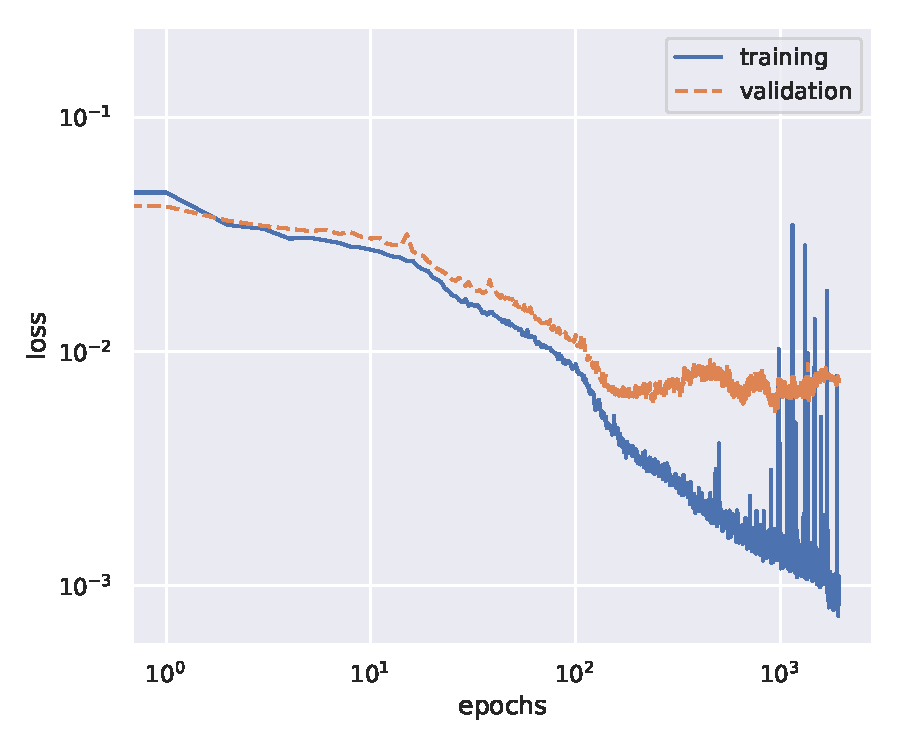
\includegraphics[width=\linewidth]{img/loss}
    \caption{Loss.}
  \end{subfigure}
  \begin{subfigure}{0.45\textwidth}
    \centering
    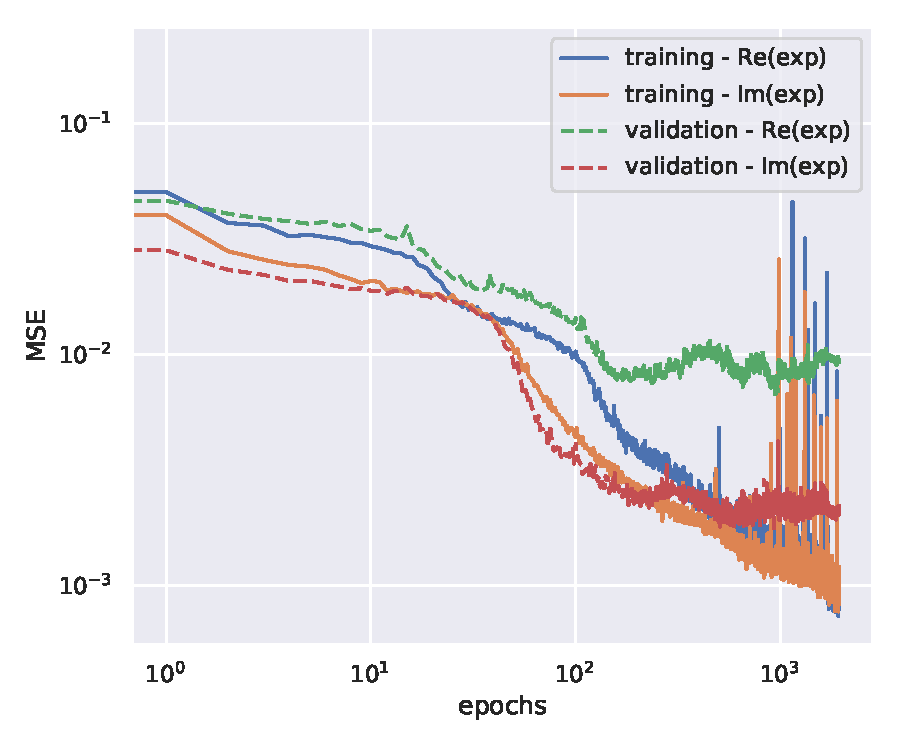
\includegraphics[width=\linewidth]{img/mse}
    \caption{\mse.}
  \end{subfigure}
  \caption{Loss function and errors (log scale).}
  \label{fig:agg:err}
\end{figure}


\subsubsection{Results}

The metrics computed on the test set are shown in \Cref{tab:agg:ann_metrics}.
The results are in general good and the coefficient of determination \rr is very high for both labels.
Comparing with the results in the validation set ($\rr = 0.94$ for $\Re(exp)$ and $\rr = 0.95$ for $\Im(exp)$), it seems that the architecture does not overfit the validation set.\footnotemark{}
\footnotetext{%
  This is in general a risk when using a single validation set.
}

\begin{table}[htbp]
  \centering
  %\resizebox{\textwidth}{!}{%
  \begin{tabular}{@{}ccc@{}}
  \toprule
       & $\Re(exp)$ & $\Im(exp)$ \\
  \midrule
  \mse & 0.02       & 0.002      \\
  \mae & 0.09       & 0.03       \\
  \rr  & 0.96       & 0.96       \\
  \bottomrule
  \end{tabular}%
  %}
  \caption{Metrics of the ANN computed on the test set.}
  \label{tab:agg:ann_metrics}
\end{table}

In fact, \Cref{fig:agg:ann_preds} shows that the agreement between predictions and true values in the test set is very good.
It also does not show signs of isolated samples producing a completely wrong predictions as for the \emph{r-SVR}.
Taking a look at the residuals we can also see that the errors are in general well distributed and do not show sign of patterns (see \Cref{fig:agg:ann_res}).

\begin{figure}[htbp]
  \centering
  \begin{subfigure}{0.45\textwidth}
    \centering
    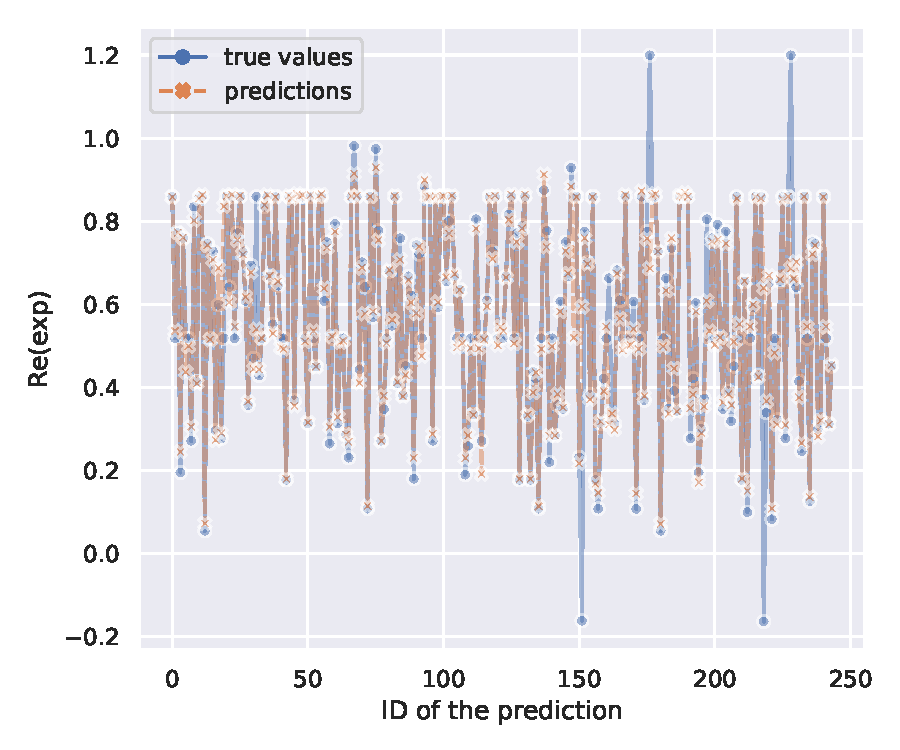
\includegraphics[width=\linewidth]{img/test_exp_re_plot}
    \caption{Real part.}
  \end{subfigure}
  \begin{subfigure}{0.45\textwidth}
    \centering
    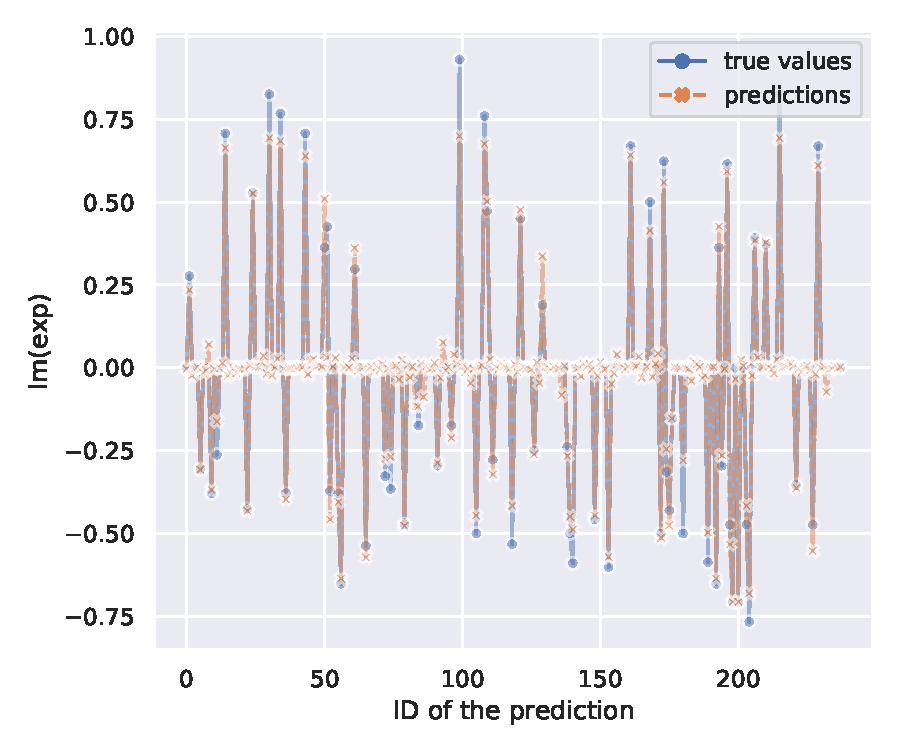
\includegraphics[width=\linewidth]{img/test_exp_im_plot}
    \caption{Imaginary part.}
  \end{subfigure}
  \caption{Predictions and true values using the \emph{ANN} model.}
  \label{fig:agg:ann_preds}
\end{figure}

\begin{figure}[htbp]
  \centering
  \begin{subfigure}{0.45\textwidth}
    \centering
    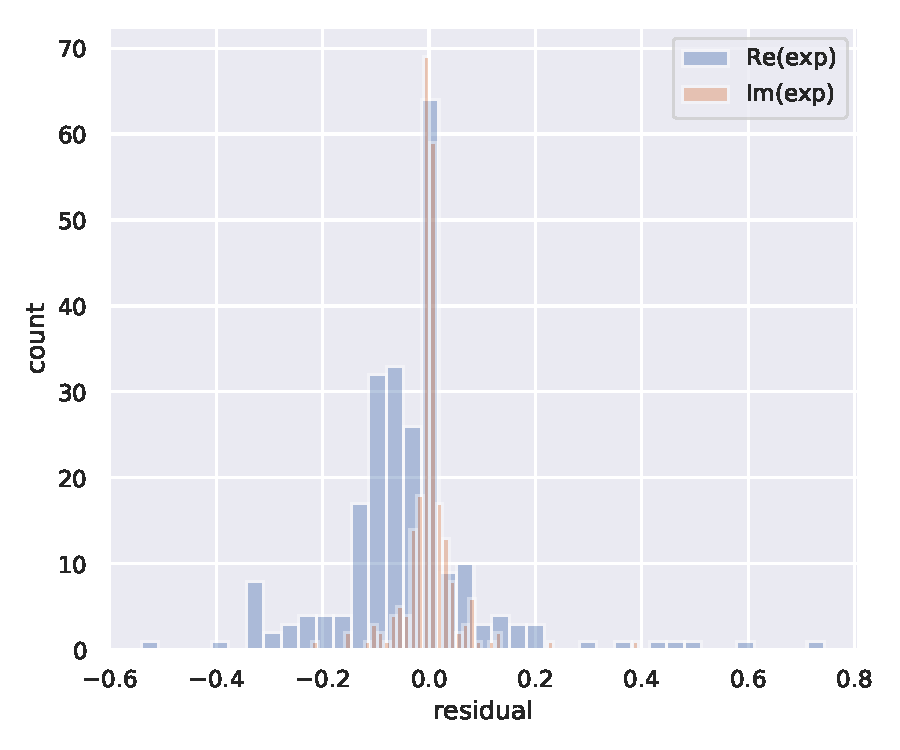
\includegraphics[width=\linewidth]{img/test_res_dist}
    \caption{Univariate distribution.}
  \end{subfigure}
  \begin{subfigure}{0.45\textwidth}
    \centering
    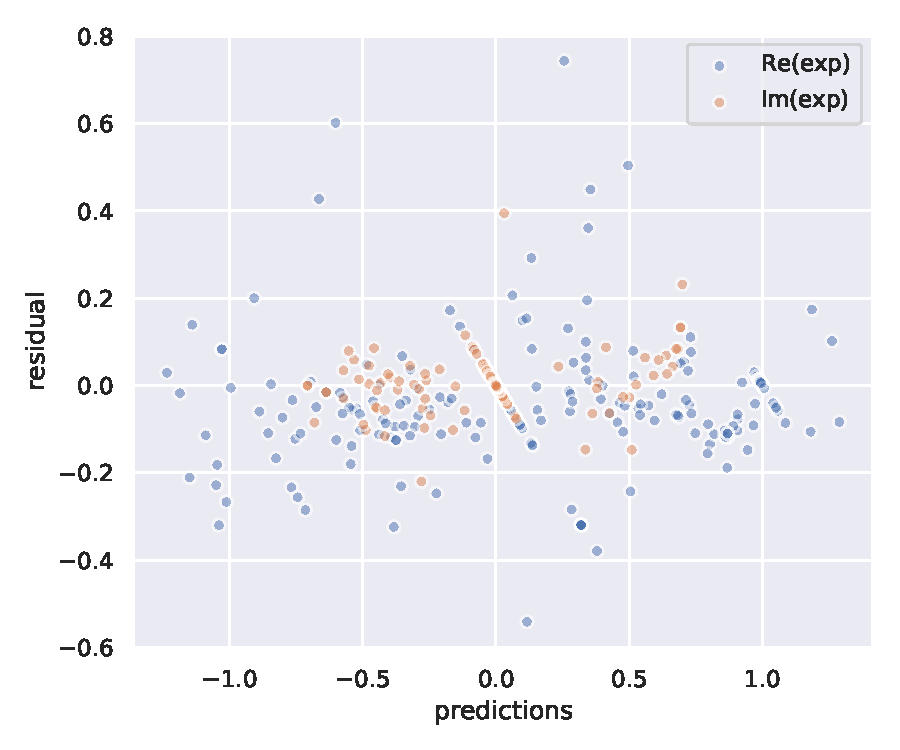
\includegraphics[width=\linewidth]{img/test_res_plot}
    \caption{Residual plot.}
  \end{subfigure}
  \caption{Residuals of the \emph{ANN} model.}
  \label{fig:agg:ann_res}
\end{figure}


\subsection{Double Lumps}

We finally use the two models trained in this section to compute the predictions on the double lumps.
We then select only the most reliable solutions (i.e.\ \texttt{weight} $< 1.5$) and compute the metrics which are summarised in \Cref{tab:agg:dlumps}.
In general it seems that the \emph{ANN} performed better even though the results are far from good.

\begin{table}[htbp]
  \centering
  \resizebox{\textwidth}{!}{%
  \begin{tabular}{@{}ccccccc@{}}
  \toprule
        & \mse $\left( \Re(exp) \right)$
        & \mse $\left( \Im(exp) \right)$
        & \mae $\left( \Re(exp) \right)$
        & \mae $\left( \Im(exp) \right)$
        & \rr $\left( \Re(exp) \right)$
        & \rr $\left( \Im(exp) \right)$ \\
  \midrule
  \emph{r-SVR} & 55 & 130   & 4   & 11   & -23   & 0.0 \\
  \emph{ANN}   & 2  & 0.004 & 1.3 & 0.05 & 0.016 & 0.0 \\
  \bottomrule
  \end{tabular}%
  }
  \caption{Metrics computed on the double lumps.}
  \label{tab:agg:dlumps}
\end{table}

Looking directly at the predictions (they are only 12 values) in \Cref{tab:agg:ann_comp}, we can see that the prediction of the real part of \texttt{exp} are in general completely off (an entire order of magnitude of difference).
However the predictions of the imaginary part have all vanishing integer part: assuming knowldge of the reality of \texttt{exp} for this model, we can in principle accept the predictions by simply truncating the results.\footnotemark{}
\footnotetext{%
  The important point is however that the model was trained on a dataset which included complex variables.
  It is not guaranteed to work also on a dataset with only real values.
  We may therefore have to adjust the predictions to account for that.
}

\begin{table}[htbp]
  \centering
  %\resizebox{\textwidth}{!}{%
  \begin{tabular}{@{}cccc@{}}
  \toprule 
  \emph{ANN} $(\Re(exp))$ &
  \emph{ANN} $(\Im(exp))$ &
  $\Re(exp)$ &
  $\Im(exp)$ \\
  \midrule
  -0.11 & 0.03 & 2.00  & 0.00 \\
  0.07  & 0.05 & -0.00 & 0.00 \\
  0.5   & 0.05 & -2.0  & 0.00 \\
  0.6   & 0.02 & 2.0   & 0.00 \\
  0.7   & 0.04 & 1.0   & 0.00 \\
  0.5   & 0.04 & -1.1  & 0.00 \\
  0.3   & 0.15 & -2.0  & 0.00 \\
  0.4   & 0.09 & -0.8  & 0.00 \\
  0.14  & 0.09 & 1.21  & 0.00 \\
  1.0   & 0.03 & 2.0   & 0.00 \\
  0.7   & 0.02 & 0.7   & 0.00 \\
  0.6   & 0.02 & 2.0   & 0.00 \\
  \bottomrule
  \end{tabular}%
  %}
  \caption{Predictions of the \emph{ANN} model.}
  \label{tab:agg:ann_comp}
\end{table}



\section{Conclusions}
In the analysis we show that \ml techniques are indeed able to make accurate predictions on lumps and the \wzw model in \sft.
In fact decision trees and \emph{ANN} models showed promising results on a model dependent basis (i.e.\ with knowledge of the underlying physics model).
In principle it seems to also be possible to merge different datasets and produce meaningful predictions using \emph{ANN} models (and \emph{r-SVR} in some cases) which displayed the best adaptivity to different datasets.

It is still not clear whether it is possible to use algorithms trained on different datasets (even coming from diverse physical models) and make accurate predictions on different data, produced by a different physical model.
However when introducing the double lumps directly in the evaluation and test sets, the \emph{ANN}s showed ability to generalise to these solutions.
As shown by the coefficient of determination \rr, the variance of the data is greatly explained by the model, which can therefore be used for predictions.



\clearpage


\printbibliography[heading=bibintoc]


\end{document}

%vim ft=tex
